%-------------------------------------------------------------------------
% info-S1-listes.tex
%-------------------------------------------------------------------------

%-------------------------------------------------------------------------
\section{Introduction}
%-------------------------------------------------------------------------
\marginpar{\footnotesize\em
\begin{fig}[Définitions de l'Académie (9)]\label{fig:dico-listes1}
{\em DONNÉE} n. f. XIIIe siècle, au sens de «~distribution, aumône~» ; XVIIIe siècle, 
comme terme de mathématiques. Participe passé féminin substantivé de donner au sens de «~indiquer, dire~».
1. Fait ou principe indiscuté, ou considéré comme tel, sur lequel se fonde un raisonnement ; 
constatation servant de base à un examen, une recherche, une découverte. 
{\em MATH.} Chacune des quantités ou propriétés mentionnées dans l'énoncé d'un problème 
et qui permettent de le résoudre.
{\em INFORM.} Représentation d'une information sous une forme conventionnelle adaptée à son exploitation.\\
\mbox{}\\
{\em COLLECTION} n. f. XIVe siècle, au sens de « amas de pus » ; XVIIe siècle, au sens moderne. 
Emprunté du latin collectio, « action de recueillir, de rassembler », 
« ce qui est recueilli ».
1. Ensemble d'objets de même sorte que l'on réunit volontairement dans 
un esprit de curiosité, ou pour leur valeur artistique, 
scientifique ou documentaire.
\end{fig}
}
Un algorithme est une suite ordonnée d'instructions qui indique la démarche à
suivre pour résoudre une série de problèmes équivalents. 
Les deux chapitres précédents concernaient la structuration des algorithmes,
soit en contrôlant le flux d'instructions à l'aide d'instructions de base
appropriées (chapitre \ref{ch:instructions}), soit en factorisant des séquences
d'instructions au sein de fonctions et procédures (chapitre \ref{ch:fonctions}).
Par contre, ils ne s'intéressaient pas explicitement aux données manipulées par ces algorithmes.
Ce sera l'objet de ce chapitre d'aborder la structuration des données manipulées
par les algorithmes.

\begin{ex}[Distance entre 2 points du plan]\label{ex:points}
Soient deux points du plan $M_1$ et $M_2$ respectivement de coordonnées $(x_1,y_1)$ et $(x_2,y_2)$.
La distance $d$ entre ces 2 points est classiquement calculée par $d = \sqrt{(x_2-x_1)^2 + (y_2-y_1)^2}$
dont on déduit l'implémentation informatique suivante :

\noindent\mbox{}\hspace*{1cm}\begin{py}{9cm}\tt
def distance(x1,y1,x2,y2):\\
\mbox{}\ \ \ \ return sqrt((x2-x1)**2 + (y2-y1)**2)
\end{py}
\hfill
\begin{py}{6cm}\tt
>>> distance(0,0,1,1)\\
1.4142135623730951
\end{py}
\end{ex}

\marginpar{\footnotesize\em
\begin{td}[Distance de 2 points de l'espace]\label{td:distance}
Définir la fonction {\tt distance} qui calcule la distance entre 2 points
$M_1$ et $M_2$ de l'espace, respectivement de coordonnées $(x_1,y_1,z_1)$ 
et $(x_2,y_2,z_2)$.
\end{td}
}
\noindent La fonction {\tt distance} précédente prend 4 arguments 
(les 4 coordonnées $x_1$, $y_1$, $x_2$, $y_2$) là où l'utilisateur de la fonction
aurait certainement préféré parler plus directement des 2 points $M_1$ et $M_2$. 
Pour cela, il faut être capable de réunir 2 par 2 les coordonnées des 2 points au 
sein d'une même collection de données (figure \ref{fig:dico-listes1}) et passer des 
points plutôt que des coordonnées. C'est ce qui est proposé dans l'implémentation 
suivante en utilisant les n-uplets de {\sc Python} où la fonction ne prend plus que 
2 arguments (les 2 points $M_1$ et $M_2$).

\noindent\mbox{}\hspace*{1cm}\begin{py}{9cm}\tt
def distance(m1,m2):\\
\mbox{}\ \ \ \ return sqrt((m2[0]-m1[0])**2 + (m2[1]-m1[1])**2)
\end{py}
\hfill
\begin{py}{6cm}\tt
>>> m1, m2 = (0,0), (1,1)\\
>>> distance(m1,m2)\\
1.4142135623730951
\end{py}
\exo{td:distance}
\vspace*{2mm}

Ce regroupement de coordonnées permet de définir la notion de point là où
ne manipulait initialement que des coordonnées. On introduit ainsi de nouveaux 
types de données.

%-------------------------------------------------------------------------
\subsection{Types de données}
%-------------------------------------------------------------------------
En informatique, une donnée est la représentation d'une information sous une forme
conventionnelle adaptée à son exploitation. Une variable est alors un objet informatique 
qui associe un nom à cette représentation (section \ref{sub:variables} page \pageref{sub:variables})
et qui, selon les langages, est implicitement ou explicitement typée.
On distingue classiquement les types de base comme les booléens (type {\tt bool}, {\tt \{False,True\}}),
les « entiers » (type {\tt int}, en fait un sous-ensemble des nombres relatifs $\Bbb Z$) et les « réels »
(type {\tt float}, en fait un sous-ensemble des nombres rationnels $\Bbb Q$) des
types structurés qui sont des regroupements de types tels que les listes (type {\tt list}, 
exemple : {\tt [0,3.14,[4,True]]}), les n-uplets (type {\tt tuple}, exemple : {\tt (0,3.14,[4,(True,8)])}
ou les dictionnaires (type {\tt dict}, exemple : {\tt \{'a': [1,2,3], 'b': 5\}}).
\marginpar{\footnotesize\em
\begin{rem} En {\sc Python}, les principaux types de base sont les booléens ({\tt bool}),
les entiers ({\tt int}), les réels ({\tt float}), les complexes ({\tt complex}), 
les chaînes de caractères ({\tt str}), les n-uplets ({\tt tuple}), les listes ({\tt list}), 
les ensembles ({\tt set}), les fichiers ({\tt file}) et les dictionnaires ({\tt dict}).
\end{rem}
}

\begin{defin}[type de données]\index[def]{type}\index{variable!type}\index{type de données}
Le type d'une variable définit l'ensemble des valeurs qu'elle peut prendre 
et l'ensemble des opérations qu'elle peut subir.
\end{defin}

D'une manière plus formelle, on définit des types abstraits de données ({\sc Tad})
\index{type abstrait de données} où les données sont considérées de manière abstraite 
indépendamment d'une implémentation dans un langage donné sur une machine particulière. 
On choisit alors une notation pour les décrire ainsi que pour décrire l'ensemble des opérations 
qu'on peut leur appliquer et les propriétés de ces opérations. Il existe plusieurs 
manières de définir un type abstrait de données qui diffèrent essentiellement
dans la façon de décrire les propriétés des opérations du type. 
\marginpar{\footnotesize\em
\begin{rem}
On pourra également consulter \cite{froidevaux} pour approfondir
cette notion de type abstrait de données, en particulier dans le cas des séquences 
et des principaux algorithmes associés de recherche et de tri.
\end{rem}
}
L'annexe \ref{tad:sequence} page \pageref{tad:sequence} propose un exemple de 
type abstrait de séquence fondé sur un formalisme logique \cite{manna}\label{cite:manna}, mais dans ce qui suit
(section \ref{sequence}) nous aborderons les séquences de manière plus pragmatique et opérationnelle.

On peut ainsi regrouper n'importe quelles données entre elles pour former un nouveau 
type de données comme :
\begin{itemize}
\item un nombre rationnel formé de 2 entiers : le numérateur et le dénominateur
	(exemple: {\tt (n,d)} pourra représenter le rationnel $n/d$), 
\item un nombre complexe formé de 2 réels : la partie réelle et la partie 
	imaginaire (exemple: {\tt (x,y)} pourra représenter le complexe $x+iy$),
\item un vecteur de l'espace formé de 3 réels : l'abscisse, l'ordonnée
	et la côte (exemple: {\tt (x,y,z)} pourra représenter le vecteur de ${\Bbb R}^3$
	de composantes $(x,y,z)$),
\item une fiche d'état civil formé de 3 chaînes de caractères et d'un entier : 
	le nom, le prénom, la nationalité et l'âge (exemple : {\tt (nom,prenom,pays,age)})
	pourra représenter l'individu {\tt nom prenom} originaire de {\tt pays} et âgé
	de {\tt age} ans.
\end{itemize}
Dans les exemples précédents, le nombre d'éléments qui composent le regroupement
est connu à l'avance (un rationnel sera toujours composé de 2 entiers, un vecteur de $\Bbb R^3$
aura toujours 3 composantes réelles\ldots). Mais ce n'est pas toujours le cas; on parlera alors 
de collections de données.

%-------------------------------------------------------------------------
\subsection{Collections}\label{sub:collections}
%-------------------------------------------------------------------------

\begin{defin}[collection de données]\index[def]{collection}\index{collection de données}
Une collection est un regroupement fini de données dont le nombre n'est pas fixé {\em a priori}.
\end{defin}

\marginpar{\footnotesize\em
\begin{fig}[Exemple de collection]\label{fig:chaussures}
Tas de chaussures\\
\centerline{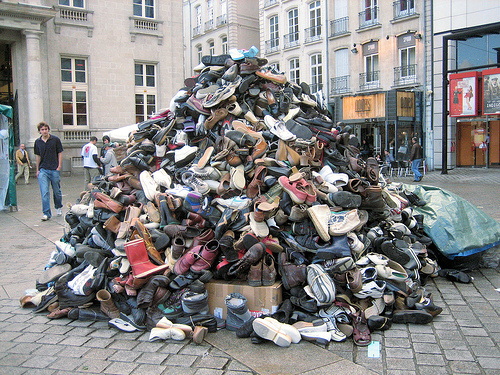
\includegraphics[width=7cm]{chaussures.jpg}}
\end{fig}
}
Ainsi les collections que l'on utilise en informatique sont des objets dynamiques. 
Le nombre de leurs éléments varie au cours de l'exécution du programme, 
puisqu'on peut y ajouter et supprimer des éléments en cours de traitement. 
Plus précisément les principales opérations que l'on s'autorise sur les collections 
sont les suivantes :  
\begin{itemize}
\item déterminer le nombre d'éléments de la collection,
\item tester l'appartenance d'un élément à la collection,
\item ajouter un élément à la collection,
\item supprimer un élément de la collection.
\end{itemize}

\begin{ex}[Tas de chaussures]\label{ex:chaussures}
Dans le tas de chaussures de la figure \ref{fig:chaussures} ci-contre, il est très facile 
d'ajouter une paire de chaussures sur le tas : il suffit de la jeter sans précaution
sur les autres chaussures. Par contre, pour supprimer une chaussure
particulière du tas, ce sera beaucoup plus difficile car il faudra d'abord la retrouver 
dans cet amas non structuré de chaussures.
\end{ex}

A l'inverse du tas de chaussures, les collections informatiques seront structurées 
pour faciliter et optimiser la recherche d'un élément en leur sein.
Les éléments peuvent être de différents types, mais les opérations
que l'on effectue sur les collections doivent être indépendantes 
des types de données des éléments.

\marginpar{\footnotesize\em
\begin{fig}[Eléments d'une séquence]\label{fig:sequence}
$$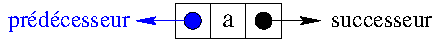
\includegraphics{sequence.pdf}$$
Exemple de séquence : main au poker
$$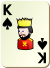
\includegraphics[width=1.25cm]{roi-pique.png}\ 
\includegraphics[width=1.25cm]{dame-pique.png}\ 
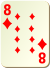
\includegraphics[width=1.25cm]{huit-carreau.png}\ 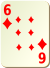
\includegraphics[width=1.25cm]{six-carreau.png}\ 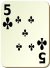
\includegraphics[width=1.25cm]{cinq-trefle.png}$$
\end{fig}
}
On distingue classiquement 3 grands types de collections : les séquences, les arbres et les graphes.

\begin{defin}[séquence]\index[def]{séquence}\index{séquence}
Une séquence est une suite ordonnée d'éléments, éventuellement vide, accessibles par leur rang dans la séquence.
\end{defin}

Dans une séquence (figure \ref{fig:sequence}), chaque élément a un prédecesseur (sauf le premier élément qui n'a pas de
prédécesseur) et un successeur (sauf le dernier élément qui n'a pas de successeur).
Une liste de noms, une main d'un jeu de cartes, une pile d'assiettes ou une file de spectateurs
sont des exemples de structures séquentielles de la vie courante.
En {\sc Python}, on utilisera 3 types de séquences : 
les chaînes de caractères (type {\tt str}, exemples : {\tt ''}, {\tt 'bonjour'}, {\tt "ça va ?"}), 
les n-uplets (type {\tt tuple}, exemples : {\tt ()}, {\tt (1,2,3)}, {\tt ('a',2,(1,2,3))})
et les listes (type {\tt list}, exemples : {\tt []}, {\tt [a,b,c,d,e]}, {\tt [1,'e',(1,2,[x,y])]}).

\marginpar{\footnotesize\em
\begin{fig}[N\oe ud d'un arbre]\label{fig:arbre}
$$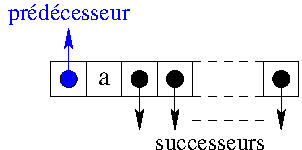
\includegraphics{arbre.pdf}$$
\end{fig}
}

\begin{defin}[arbre]\index[def]{arbre}\index{arbre}
Un arbre est une collection d'éléments, appelés « n\oe uds », organisés de façon hiérarchique à partir 
d'un n\oe ud particulier, appelé la « racine » de l'arbre.
\end{defin}

Dans un arbre (figure \ref{fig:arbre}), chaque élément a un seul prédecesseur (sauf la racine de l'arbre 
qui n'a pas de prédecesseur) et peut avoir plusieurs successeurs (on appelle « feuille » de l'arbre un n\oe ud qui 
n'a pas de successeurs). L'arbre est dit « $n$-aire » si chaque n\oe ud a au plus $n$ successeurs;
si $n=2$, on parle d'arbre binaire.
Les répertoires d'un système d'exploitation en informatique,
la classification des espèces animales en biologie ou
le tableau final d'un tournoi de tennis
constituent des exemples connus de structures arborescentes.

\begin{ex}[Tableau final d'un tournoi de football]\label{ex:euro2000}
Dans l'exemple de la figure \ref{fig:euro2000} ci-contre, les n\oe uds de
l'arbre sont les rencontres (exemples: le quart de finale Portugal/Turquie,
la demi-finale Pays-Bas/Italie). Il s'agit d'un arbre binaire
dont la racine est la finale France/Italie. Les quarts de finale sont les feuilles
de cet arbre binaire.
\end{ex}
\marginpar{\footnotesize\em\vspace*{-4cm}
\begin{fig}[Exemple d'arbre]\label{fig:euro2000}
Tableau final de l'Euro 2000 de football
$$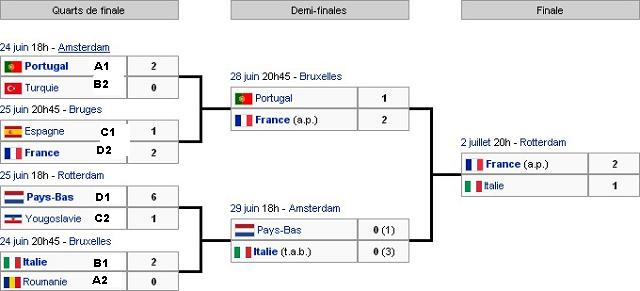
\includegraphics[width=7cm]{euro-2000.jpg}$$
\end{fig}
\begin{fig}[Sommet d'un graphe]\label{fig:graphe}
$$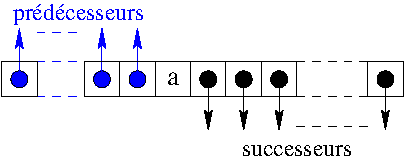
\includegraphics{graphe.pdf}$$
\end{fig}
\begin{fig}[Schéma d'un graphe orienté]\label{fig:schemaGraphe}
$$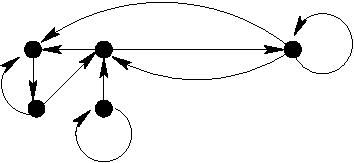
\includegraphics{schemaGraphe.pdf}$$
\end{fig}
}
En {\sc Python}, les ensembles (type {\tt set}) et les dictionnaires (type {\tt dict}) 
sont implémentés sous forme d'arbres.

\begin{defin}[graphe]\index[def]{graphe}\index{graphe}
Un graphe est une collection d'éléments, appelés « sommets », et de relations entre ces sommets.
\end{defin}

Dans un graphe (figure \ref{fig:graphe}), chaque élément peut avoir plusieurs prédécesseurs et plusieurs successeurs.
Un même élément peut être à la fois prédécesseur et successeur d'un autre sommet (y compris de lui-même).
On parle de « graphe orienté » lorsque les relations entre sommets sont des paires ordonnées de sommets
(les relations sont alors appelées « arcs » du graphe); on parle de « graphe non orienté~» si ce sont des paires
non orientées (les relations sont alors appelées « arêtes » du graphe).
Un graphe est facilement représentable par un schéma (figure \ref{fig:schemaGraphe})
où les sommets sont des points et les arcs, des flèches entre
deux points (ou les arêtes, des traits entre deux points).
Un circuit électronique, une toile d'araignée ou internet sont des exemples
de tels graphes.

Les graphes permettent de manipuler plus facilement des objets et leurs
relations. L'ensemble des
techniques et outils mathématiques mis au point en « Théorie des Graphes »
permettent de démontrer certaines propriétés des graphes, d'en déduire des
méthodes de résolution, des algorithmes\ldots


\begin{ex}[Carte routière]\label{ex:finistere}
Dans la carte routière de la figure \ref{fig:finistere}, les villes sont les sommets
d'un graphe non orienté dont les arêtes sont les routes qui mènent d'une ville à l'autre.
Sur un tel graphe, on peut se poser des questions telles que :
\begin{itemize}
\item Quel est le plus court chemin (en distance ou
               en temps) pour se rendre d'une ville à une
               autre ?
\item Comment optimiser le circuit d'un voyageur de commerce de telle manière qu'il passe 
	une et une seule fois par toutes les villes de son secteur ?
\end{itemize}       
\end{ex}
\marginpar{\footnotesize\em\vspace*{-3cm}
\begin{fig}[Exemple de graphe]\label{fig:finistere}
Carte routière du Finistère Nord
$$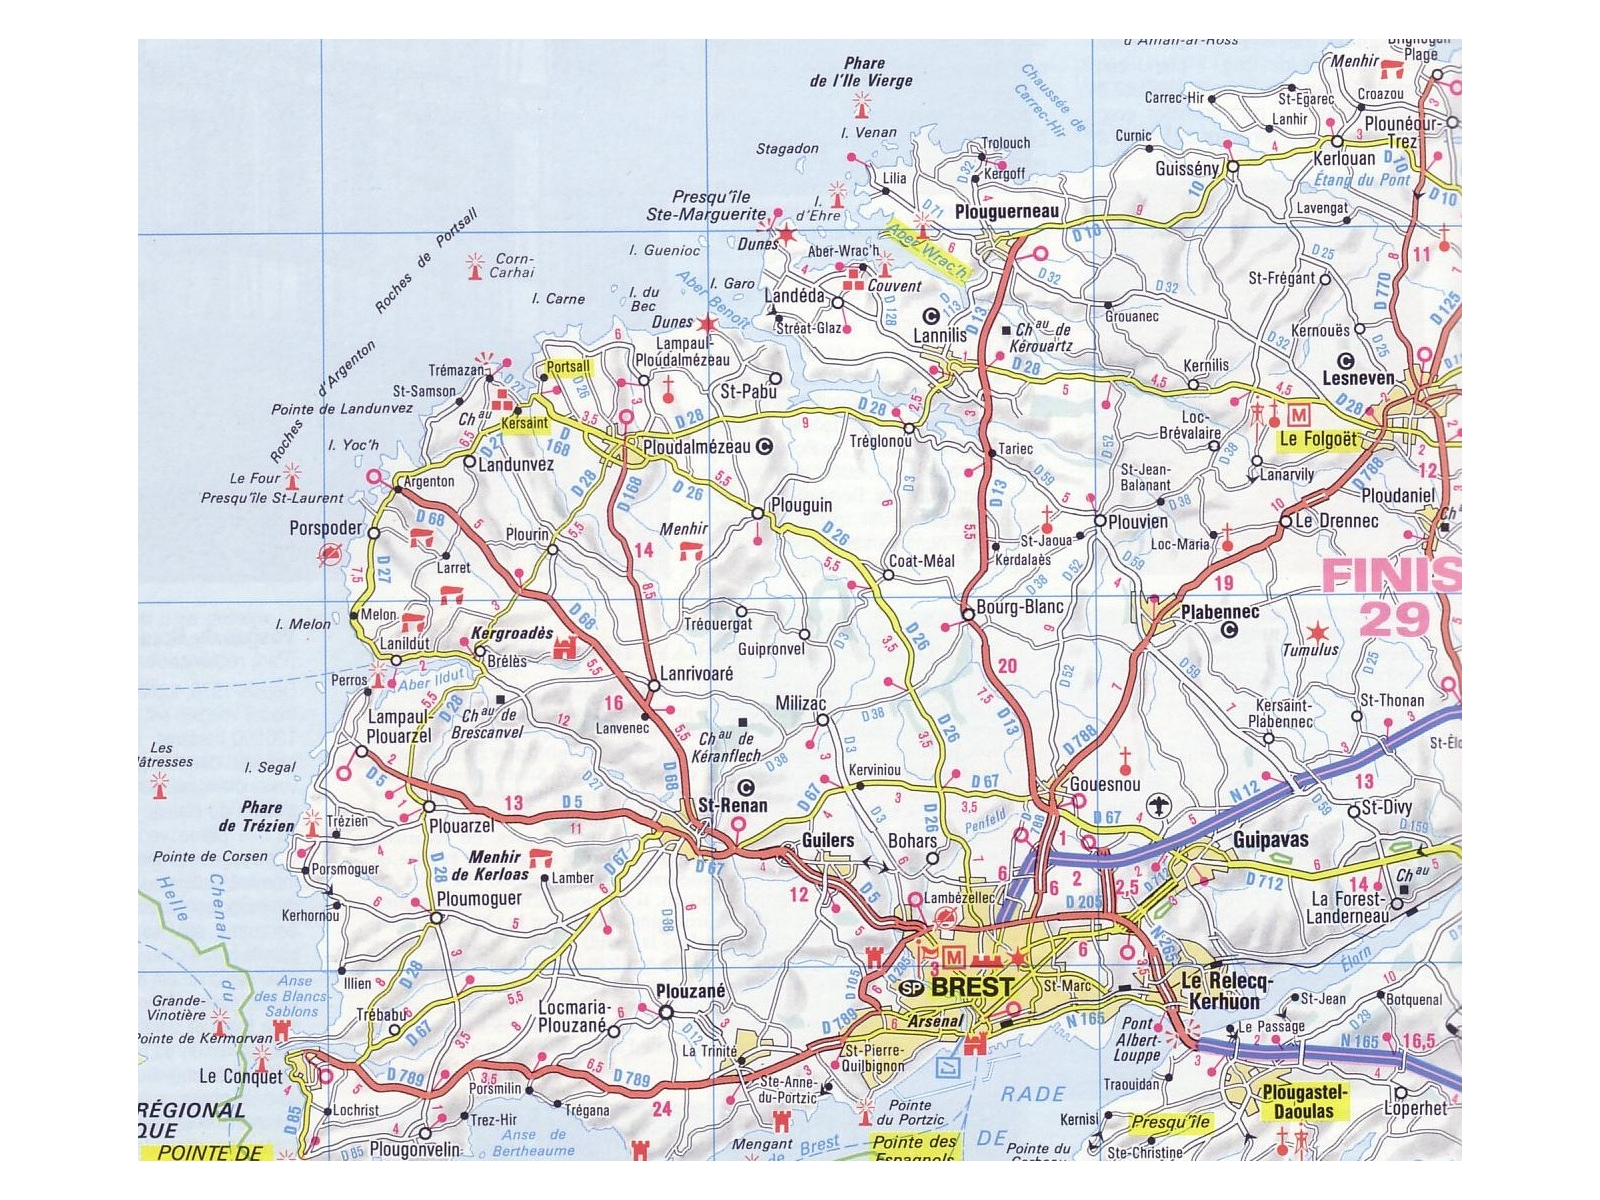
\includegraphics[width=7.5cm]{finistere-nord.jpg}$$
\end{fig}
\begin{rem} Attention ! Par convention, les indices des éléments dans une séquence commencent à {\tt 0}.
Le premier élément a pour indice {\tt 0} ({\tt s[0]}), le deuxième l'indice {\tt 1}
({\tt s[1]}), le troisième l'indice {\tt 2} ({\tt s[2]}) et ainsi de suite jusqu'au 
dernier qui a l'indice {\tt n-1} ({\tt s[n-1]}) si {\tt n} est le nombre d'éléments 
dans la séquence ({\tt n == len(s)}).
\end{rem}
\begin{rem} 
La section \ref{python:listes} page \pageref{python:listes} présente les principales opérations 
sur les séquences en {\sc Python}.
\end{rem}
}

Dans ce chapitre, nous ne nous intéresserons qu'aux structures linéaires : les séquences.
Les structures arborescentes et les graphes seront abordés à partir du semestre 4 dans 
les cours d'informatique
de l'ENIB.

%-------------------------------------------------------------------------
\section{Séquences}\label{sequence}
%-------------------------------------------------------------------------
Comme en {\sc Python}, nous distinguerons ici les n-uplets (type {\tt tuple}), les 
chaînes de caractères (type {\tt str}) et les listes (type {\tt list})
comme autant de variantes de séquences.
Quelle que soit la variante considérée, il sera toujours possible de 
déterminer le type ({\tt type(s)}) et la longueur ({\tt len(s)}) d'une séquence {\tt s}, 
de tester l'appartenance d'un élément {\tt x} à la séquence {\tt s} ({\tt x in s}), 
d'accéder à un élément par son rang {\tt i} dans la séquence ({\tt s[i]})
et de concaténer 2 séquences {\tt s1} et {\tt s2} ({\tt s1 + s2}).

\noindent\mbox{}\hspace*{1cm}\begin{py}{4cm}\tt
>>> s = 1,7,2,4\\
>>> type(s)\\
<type 'tuple'>\\
>>> len(s)\\
4\\
>>> 3 in s\\
False\\
>>> s[1]\\
7\\
>>> s + (5,3)\\
(1, 7, 2, 4, 5, 3)
\end{py}
\hfill
\begin{py}{4cm}\tt
>>> s = '1724'\\
>>> type(s)\\
<type 'str'>\\
>>> len(s)\\
4\\
>>> '3' in s\\
False\\
>>> s[1]\\
'7'\\
>>> s + '53'\\
'172453'
\end{py}
\hfill
\begin{py}{4cm}\tt
>>> s = [1,7,2,4]\\
>>> type(s)\\
<type 'list'>\\
>>> len(s)\\
4\\
>>> 3 in s\\
False\\
>>> s[1]\\
7\\
>>> s + [5,3]\\
\mbox{}[1, 7, 2, 4, 5, 3]
\end{py}
\vspace*{2mm}

Les variantes {\tt tuple}, {\tt str} et {\tt list} diffèrent par leur syntaxe et
par le fait qu'une liste est modifiable alors que les n-uplets et les 
chaînes de caractères ne le sont pas, au sens où il n'est pas possible de modifier 
un élément individuel d'une chaîne ou d'un n-uplet.

\noindent\mbox{}\hspace*{1cm}\begin{py}{4cm}\tt
>>> s = 1,7,2,4\\
>>> type(s)\\
<type 'tuple'>\\
>>> s[1] = 3\\
{\color{red}
Traceback ...\\
TypeError: 'tuple' object does not support item assignment
}\\
>>> s[1]\\
7
\end{py}
\hfill
\begin{py}{4cm}\tt
>>> s = '1724'\\
>>> type(s)\\
<type 'str'>\\
>>> s[1] = '3'\\
{\color{red}
Traceback ...\\
TypeError: 'str' object does not support item assignment
}\\
>>> s[1]\\
7
\end{py}
\hfill
\begin{py}{4cm}\tt
>>> s = [1,7,2,4]\\
>>> type(s)\\
<type 'list'>\\
>>> s[1] = 3\\
>>> s\\
\mbox{}[1, 3, 2, 4]\\
>>> s[1]\\
3
\end{py}

%-------------------------------------------------------------------------
\subsection{N-uplets}
%-------------------------------------------------------------------------
\begin{defin}[n-uplet]\index[def]{n-uplet}\index{séquence!n-uplet}\index{n-uplet}
Un n-uplets est une séquence non modifiable d'élé\-ments.
\end{defin}
On parle de singleton quand $n=1$, de paire quand $n=2$, de triplet pour $n=3$, 
de quadruplet pour $n=4$\dots\ et plus généralement de n-uplet.

D'un point de vue syntaxique, un n-uplet est une suite d'éléments
séparés par des virgules. Bien que cela ne soit pas nécessaire, il est  
conseillé de mettre un n-uplet en évidence en l'enfermant dans une paire de parenthèses, 
comme {\sc Python} le fait lui-même.
Par ailleurs, il faut toujours au moins une virgule pour définir un n-uplet, sauf pour le n-uplet vide {\tt ()}.

\marginpar{\footnotesize\em
\begin{td}[Opérations sur les n-uplets]\label{td:n-uplet}\index[td]{opérations sur les n-uplets}
Donner un exemple d'utilisation de chacune des opé\-ra\-tions  
sur les n-uplets décrites dans le tableau de la page \pageref{tab:sequences}.
\end{td}
}
\noindent\mbox{}\hspace*{1cm}\begin{py}{4cm}\tt
>>> s = ()\\
>>> type(s)\\
<type 'tuple'>\\
>>> s = 1,7,2,4\\
>>> type(s)\\
<type 'tuple'>\\
>>> s\\
(1, 7, 2, 4)
\end{py}
\hfill
\begin{py}{4cm}\tt
>>> s = (5)\\
>>> type(s)\\
<type 'int'>\\
>>> s = (5,)\\
>>> type(s)\\
<type 'tuple'>\\
>>> s = (5,)+()+(6,7,9)\\
>>> s\\
(5, 6, 7, 9)
\end{py}
\hfill
\begin{py}{4cm}\tt
>>> s = (5,6,7,9)\\
>>> s[1\char`:3]\\
(6, 7)\\
>>> s[1\char`:]\\
(6, 7, 9)\\
>>> s[\char`:2]\\
(5, 6)\\
>>> s[-2\char`:]\\
(7, 9)
\end{py}\\
\exo{td:n-uplet}

\vspace*{2mm}

Les n-uplets sont souvent utilisés pour regrouper sous une même variable
plusieurs variables logiquement reliées entre elles comme dans l'exemple
des points du plan de l'exemple \ref{ex:points} page~\pageref{ex:points}.
Ils servent également à retourner plusieurs objets dans une fonction
comme dans les exemples de la fonction standard {\tt divmod} de la section
\ref{python:fonctions} page \pageref{python:fonctions} ou encore des 
définitions de courbes paramétriques du TD \ref{td:traces} page 
\pageref{td:traces}.
\exo{td:pgcdppcm}

\marginpar{\footnotesize\em
\begin{td}[Pgcd et ppcm de 2 entiers (2)]\label{td:pgcdppcm}\index[td]{pgcd et ppcm de 2 entiers}\hfill voir TD \ref{td:pgcd}
Définir une fonction qui calcule le pgcd et le ppcm de 2 entiers $a$ et $b$.
\end{td}
}

%-------------------------------------------------------------------------
\subsection{Chaînes de caractères}
%-------------------------------------------------------------------------
\begin{defin}[chaîne de caractères]\index[def]{chaîne de caractères}\index{séquence!chaîne de caractères}\index{chaîne de caractères}
Une chaîne de caractères est une séquence non modifiable de caractères.
\end{defin}

\marginpar{\footnotesize\em
\begin{rem} 
L'ordinateur stocke toutes les données sous forme numérique
(ensemble de bits). En particulier, les caractères ont un équivalent numérique : 
le code ASCII ({\em American Standard Code for Information Interchange}). 
Le code ASCII de base code les caractères sur 7 bits (128 caractères : de 0 à 127,
voir section \ref{ascii} page \pageref{ascii}).

En {\sc Python}, les fonctions standard {\tt ord} et {\tt chr} permettent
de passer du caractère au code ASCII et inversement.

\noindent\mbox{}\hspace*{1cm}\begin{py}{3cm}\tt
>>> ord('e')\\
101\\
>>> ord('é')\\
233
\end{py}
\hfill
\begin{py}{3cm}\tt
>>> chr(101)\\
'e'\\
>>> chr(233)\\
'é'
\end{py}
\end{rem}
}
D'un point de vue syntaxique, une chaîne de caractères est une suite quelconque de 
caractères délimitée soit par des apostrophes (simple {\em quotes} : {\tt '\ldots'}), 
soit par des guillemets (double {\em quotes} : {\tt "\ldots"}).
On peut ainsi utiliser des guillemets pour délimiter une chaîne dans laquelle il y a des
apostrophes (exemple : {\tt "c'est ça !"}), ou utiliser des apostrophes pour délimiter 
une chaîne qui contient des guillemets (exemple : {\tt '"hello" dit-il.'}).
Pour sa part, le caractère {\em antislash} ({\tt \char`\\}) permet 
d'écrire sur plusieurs lignes une chaîne qui serait trop longue pour
tenir sur une seule ou bien d'insérer, à l'intérieur d'une chaîne, un certain nombre de caractères
spéciaux comme les sauts à la ligne ({\tt \char`\\n}), les apostrophes ({\tt \char`\\'}), 
les guillemets ({\tt \char`\\"})\ldots\ 
En {\sc Python}, pour insérer plus aisément des caractères spéciaux dans une chaîne, 
sans faire usage de l'{\em antislash}, ou pour faire accepter l'{\em antislash} lui-même 
dans la chaîne, on peut délimiter la chaîne à l'aide 
de triples apostrophes ({\tt '''\ldots'''}) ou de triples guillemets ({\tt """\ldots"""}).

\marginpar{\footnotesize\em
\begin{td}[Opérations sur les chaînes]\label{td:chaine}\index[td]{opérations sur les chaînes de caractères}
Donner un exemple d'utilisation de chacune des opé\-ra\-tions  
sur les chaînes de caractères décrites dans le tableau de la page \pageref{tab:chaines}.
\end{td}
}
\noindent\mbox{}\hspace*{1cm}\begin{py}{6.5cm}\tt
>>> s = 'chaîne entrée sur \char`\\ \\
... plusieurs lignes'\\
>>> s\\
'chaîne entrée sur plusieurs lignes'\\
>>> s = 'chaîne entrée \char`\\n sur 1 ligne'\\
>>> print(s)\\
chaîne entrée\\
\mbox{}\ sur 1 ligne
\end{py}
\hfill
\begin{py}{6.5cm}\tt
>>> s = 'c\char`\\'est ça \char`\\"peuchère\char`\\"'\\
>>> s\\
'c\char`\\'est ça "peuchère"'\\
>>> print(s)\\
c'est ça "peuchère"\\
>>> s = ''' a ' \char`\\\ " \char`\\n z '''\\
>>> s\\
' a \char`\\' \char`\\\char`\\\ " \char`\\n z '
\end{py}\\
\exo{td:chaine}

\vspace*{2mm}

On accède aux caractères individuels d'une chaîne de caractères par leur rang dans la chaîne,
un caractère individuel étant vu lui-même comme une chaîne à un seul caractère.

\noindent\mbox{}\hspace*{1cm}\begin{py}{6.5cm}\tt
>>> s = 'des caractères'\\
>>> s[9]\\
't'\\
>>> for c in s: print(c),\\
... \\
d e s \  c a r a c t è r e s
\end{py}
\hfill
\begin{py}{6.5cm}\tt
>>> s[4\char`:9]\\
'carac'\\
>>> s[len(s)-1]\\
's'\\
>>> s[\char`:4] + 'mo' + s[9] + s[-1]\\
'des mots'
\end{py}\\
\exo{td:inverser}

Les chaînes de caractères, et leurs opérations associées, sont évidemment très utiles pour manipuler du texte
comme peut le faire un traitement de textes par exemple.
\exo{td:wc}

\marginpar{\footnotesize\em
\begin{td}[Inverser une chaîne]\label{td:inverser}\index[td]{inverser une chaîne}
Définir une fonction qui crée une copie d'une chaîne en inversant l'ordre des caractères.

\noindent\mbox{}\hspace*{1cm}\begin{py}{6cm}\tt
>>> inverser('inverser')\\
'resrevni'
\end{py}
\end{td}

\begin{td}[Caractères, mots, lignes d'une chaîne]\label{td:wc}\index[td]{caractères, mots, lignes d'une chaîne}
Définir une fonction qui compte le nombre de caractères, le nombre de mots et le nombres de lignes
d'une chaîne de caractères.
\end{td}
}

%-------------------------------------------------------------------------
\subsection{Listes}
%-------------------------------------------------------------------------
\marginpar{\footnotesize\em
\begin{fig}[Définitions de l'Académie (10)]\label{fig:dico-listes2}
\mbox{}\\
{\em LISTE} n. f. XVIe siècle. Emprunté de l'italien lista, de même sens.
Suite ordonnée de noms, de mots, de chiffres, de nombres, de symboles, etc.
\end{fig}
}
\begin{defin}[liste]\index[def]{liste}\index{séquence!liste}\index{liste}
Une liste est une séquence modifiable d'éléments.
\end{defin}

D'un point de vue syntaxique, une liste est une suite d'éléments
séparés par des virgules et encadrée par des crochets ({\tt [\ldots]}).
On accède aux éléments individuels d'une liste comme pour une chaîne de caractères
ou un n-uplet mais, contrairement aux chaînes et aux n-uplets, on peut modifier
chaque élément d'une liste individuellement.

\marginpar{\footnotesize\em
\begin{td}[Opérations sur les listes (1)]\label{td:listes1}\index[td]{opérations sur les listes}
Donner un exemple d'utilisation de chacune des opé\-ra\-tions  
sur les listes décrites dans le tableau de la page \pageref{tab:listes}.
\end{td}
}
\noindent\mbox{}\hspace*{1cm}\begin{py}{6.5cm}\tt
>>> s = [1,3,5,7]\\
>>> s[2]\\
5\\
>>> s[len(s)-1]\\
7\\
>>> for c in s: print(c),\\
... \\
1 3 5 7
\end{py}
\hfill
\begin{py}{6.5cm}\tt
>>> s[1\char`:3]\\
\mbox{}[3,5]\\
>>> s[1\char`:3] = [2,4]\\
>>> s\\
\mbox{}[1, 2, 4, 7]\\
>>> s[len(s)\char`:len(s)] = [8,9]\\
>>> s\\
\mbox{}[1, 2, 4, 7, 8, 9]
\end{py}\\
\exo{td:listes1}

\vspace*{2mm}

Pour créer une liste, on peut explicitement le faire {\em à la main}, comme ci-dessus
avec l'instruction {\tt s = [1,3,5,7]}, mais ce n'est raisonnable que pour de 
petites listes. On peut également utiliser la fonction prédéfinie {\tt range}
pour génèrer une liste d'entiers successifs 
(voir section \ref{sub:parcours} page \pageref{sub:parcours}). 
Si {\tt range} est appelée avec un seul argument, la liste contiendra un nombre de 
valeurs égal à l'argument fourni, en commençant à partir de {\tt 0} 
({\tt range(n)} génère les nombres de {\tt 0} à {\tt n-1} : {\tt [0,1,2,\ldots,n-1]}).
On peut aussi utiliser {\tt range} avec 2 ou 3 arguments : {\tt range(debut,fin,pas)},
{\tt debut} et {\tt pas} étant optionnels.
L'argument {\tt debut} est la première valeur à générer ({\tt debut = 0} par défaut), 
l'argument {\tt pas} est l'incrément ({\tt pas = +1} par défaut) qui permet
de passer d'une valeur à la suivante ({\tt [debut, debut + pas, debut + 2*pas,\ldots]})
et l'argument obligatoire {\tt fin} est la borne maximale (valeur {\tt fin} exclue) des nombres à générer.

\noindent\mbox{}\hspace*{1cm}\begin{py}{6.5cm}\tt
>>> range(5)\\
\mbox{}[0, 1, 2, 3, 4]\\
>>> range(2,5)\\
\mbox{}[2, 3, 4]
\end{py}
\hfill
\begin{py}{6.5cm}\tt
>>> range(0,5,2)\\
\mbox{}[0, 2, 4]\\
>>> range(5,0,-2)\\
\mbox{}[5, 3, 1]
\end{py}
\vspace*{2mm}

\noindent La fonction {\tt range} est fréquemment utilisée dans les boucles pour répéter 
un nombre de fois connu à l'avance les instructions de la boucle. Mais d'une manière 
plus générale, on utilisera les fonctions d'ajout ({\tt append}) ou d'insertion
({\tt insert}) d'éléments pour créer de nouvelles listes par programme.

On dispose en effet pour les listes des opérations préconisées pour les collections
(section \ref{sub:collections} page \pageref{sub:collections}) et que l'on 
retrouve dans le tableau de la page \pageref{tab:listes} :
\marginpar{\footnotesize\em\vspace*{-4cm}
\begin{td}[Opérations sur les listes (2)]\label{td:listes2}
Vérifier que les opérations suivantes sont équivalentes deux à deux :
$$\begin{tabular}{l@{ et }l}
{\tt del s[i\char`:j]}	& {\tt s[i\char`:j] = []}\\
{\tt s.append(x)}	& {\tt s[len(s)\char`:len(s)] = [x]}\\
{\tt s.extend(x)}      	& {\tt s[len(s)\char`:len(s)]= x}\\
{\tt s.insert(i,x)}	& {\tt s[i\char`:i] = [x]}\\
{\tt s.remove(x)}	& {\tt del s[s.index(x)]}\\
{\tt s.pop(i)}		& {\tt x = s[i]; del s[i]; return x}\\
\end{tabular}$$
\end{td}
\begin{td}[Sélection d'éléments]\label{td:collect}\index[td]{sélection d'éléments}
\begin{enumerate}
\item Définir une fonction qui crée une liste {\tt t} composée des éléments d'une autre 
	liste {\tt s} qui vérifient une certaine condition {\tt p} ({\tt p(s[i]) == True}).
\item Définir une fonction qui supprime d'une liste {\tt s} les éléments qui ne vérifient
	pas une certaine condition {\tt p}.
\end{enumerate}
\end{td}
\begin{rem}En \python, l'instruction spéciale, ap\-pelée {\em list comprehension} :\\
{\tt \mbox{}\ \ t = [expression for element in sequence]}\\
est équivalente à :\\
{\tt \mbox{}\ \ t = []\\
\mbox{}\ \ for element in sequence: \\
\mbox{}\ \ \ \ \ \ t.append(expression)}\\
Exemples : \\
\begin{py}{3.75cm}\tt
>>> s = [1,2,3]\\
>>> t = [c for c in s]\\
>>> t\\
\mbox{}[1, 2, 3]
\end{py}
\hfill
\begin{py}{4cm}\tt
>>> s = [1,2,3]\\
>>> y = [c\%2 for c in s]\\
>>> y\\
\mbox{}[1, 0, 1]
\end{py}
\end{rem}
}
\begin{itemize}
\item déterminer le nombre d'éléments de la liste {\tt s},\hfill{\tt len(s)}
\item tester l'appartenance d'un élément {\tt x} à la liste {\tt s},\hfill{\tt x in s}
\item ajouter un élément {\tt x} à la liste {\tt s},\hfill{\tt s.append(x)}\\
	et plus généralement insérer un élément {\tt x} au rang {\tt i}
	dans la liste {\tt s},\hfill{\tt s.insert(i,x)}
\item supprimer l'élément de rang {\tt i} de la liste {\tt s}.\hfill{\tt del(s[i])}
\end{itemize}
\exo{td:listes2}

On dispose également de quelques autres opérations particulièrement efficaces telles 
que compter les occurences ({\tt s.count(x)}), retrouver le rang de la première occurence
d'un élément ({\tt s.index(x)}), inverser une liste ({\tt s.reverse()}) ou trier une liste
({\tt s.sort()}).
\exo{td:collect}

\noindent\mbox{}\hspace*{1cm}\begin{py}{6.5cm}\tt
>>> s = [1,2,1,1,2]\\
>>> s.count(1)\\
3\\
>>> s.index(2)\\
1
\end{py}
\hfill
\begin{py}{6.5cm}\tt
>>> s.reverse()\\
>>> s\\
\mbox{}[2, 1, 1, 2, 1]\\
>>> s.sort()\\
\mbox{}[1, 1, 1, 2, 2]
\end{py}\\

\vspace*{2mm}

Comme nous l'avons déjà évoqué à l'occasion du passage des paramètres par référence
lors de l'appel d'une fonction (section \ref{sub:passage} page \pageref{sub:passage}), 
le nom du liste est en fait une référence sur cette liste. Ainsi, si {\tt s} est une liste,
l'instruction {\tt t = s} ne fait que copier la référence de la liste et non la liste
elle-même : {\tt t} devient un alias de {\tt s} et toute modification d'un élément de {\tt t}
(ou de {\tt s}) modifie également {\tt s} (ou {\tt t}). 
Pour copier la liste, il faudra d'une 
manière ou d'une autre copier les éléments un par un, comme 
ci-dessous à droite par exemple.

\noindent\mbox{}\hspace*{1cm}\begin{py}{6.5cm}\tt
>>> s = [1,2,3]\\
>>> t = s\\
>>> t[0] = 9\\
>>> t\\
\mbox{}[9, 2, 3]\\
>>> s\\
\mbox{}[9, 2, 3]
\end{py}
\hfill
\begin{py}{6.5cm}\tt
>>> s = [1,2,3]\\
>>> t = []\\
>>> t[\char`:0] = s[0\char`:]\\
>>> t\\
\mbox{}[1, 2, 3]\\
>>> t[0] = 9\\
>>> t\\
\mbox{}[9, 2, 3]\\
>>> s\\
\mbox{}[1, 2, 3]
\end{py}
\vspace*{2mm}

\marginpar{\footnotesize\em\vspace*{-5cm}
\begin{fig}[Définitions de l'Académie (11)]\label{fig:dico-listes3}
\mbox{}\\
{\em FILE} n. f. XVe siècle. Déverbal de filer.
Suite de personnes ou de choses placées les unes derrière les autres sur une même ligne.\\
\mbox{}\\
{\em PILE} n. f. Ensemble d'objets de même sorte placés les uns sur les autres.
\end{fig}
\begin{fig}[Piles d'assiettes]\label{fig:assiettes}
$$
\includegraphics{assiettes.jpg}$$
\end{fig}
\begin{fig}[Files d'attente à un péage]\label{fig:attente}
$$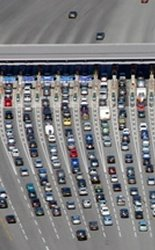
\includegraphics[height=6cm]{attente.jpg}$$
\end{fig}
}

%-------------------------------------------------------------------------
\subsection{Piles et files}\label{pilefile}
%-------------------------------------------------------------------------
Dans de nombreux cas, les seules opérations à effectuer sur les 
listes sont des insertions et des suppressions aux extrémités de la liste.
C'est le cas en particulier des piles ({\em stack}) et des files ({\em queue}).

\begin{ex}[Pile d'assiettes]\label{ex:assiettes}
Dans une pile d'assiettes (figure \ref{fig:assiettes}),
on ajoute des assiettes au sommet de la pile, et on les récupère dans l'ordre inverse, 
en commençant par la dernière ajoutée.
\end{ex}

\begin{defin}[pile]\index[def]{pile}\index{séquence!pile}\index{pile}
Une pile est une séquence dans laquelle on ne peut ajouter et supprimer un élément
qu'à une seule extrémité : le « sommet » de la pile.
\end{defin}

Dans le cas des piles, on ajoute (on empile) et on supprime (on dépile) à une
seule extrémité. Une pile est ainsi basée sur le principe
« dernier arrivé, premier sorti » ({\sc Lifo}\index{séquence!{{\sc Lifo}}} : {\em Last In, First Out}) : 
le dernier élément ajouté au sommet de la pile sera le premier à être récupéré. 
Les seules opérations nécessaires pour une pile sont ainsi :
\begin{itemize}
\item tester si la pile {\tt p} est vide,\hfill{\tt ok = emptyStack(p)}
\item accéder au sommet {\tt x} de la pile {\tt p},\hfill{\tt x = topStack(p)}
\item empiler un élément {\tt x} au sommet de la pile {\tt p},\hfill{\tt pushStack(p,x)}
\item dépiler l'élément {\tt x} qui se trouve au sommet de la pile {\tt p}.\hfill{\tt x = popStack(p)}
\end{itemize}
\exo{td:pile}

\marginpar{\footnotesize\em
\begin{td}[Opérations sur les piles]\label{td:pile}\index[td]{opérations sur les piles}
Définir les 4 opérations sur les piles définies ci-contre~: {\tt emptyStack}, {\tt topStack},
{\tt pushStack} et {\tt popStack}. On empilera et dépilera à la fin de la liste qui
sert à stocker les éléments de la pile.
\end{td}
}
\begin{ex}[File d'attente de voitures]\label{ex:attente}
A un péage (figure \ref{fig:attente}), la première voiture à être entrée dans une file d'attente
sera la première sortie de la file.
\end{ex}

\begin{defin}[file]\index[def]{file}\index{séquence!file}\index{file}
Une file est une séquence dans laquelle on ne peut ajouter un élément qu'à une seule extrémité 
et ne supprimer un élément qu'à l'autre extrémité : la « tête » de la file.
\end{defin}

\marginpar{\footnotesize\em
\begin{td}[Opérations sur les files]\label{td:file}\index[td]{opérations sur les files}
Définir les 4 opérations sur les files définies ci-contre~: {\tt emptyQueue}, {\tt topQueue},
{\tt pushQueue} et {\tt popQueue}. On enfilera en début de liste et on défilera à la fin de la liste qui
sert à stocker les éléments de la file.
\end{td}
\begin{fig}[Définitions de l'Académie (12)]\label{fig:dico-listes4}
\mbox{}\\
{\em MATRICE} n. f. XIIIe siècle. Emprunté du latin matrix, matricis, « reproductrice », 
dérivé de mater, « mère ».
MATH. Ensemble ordonné de nombres algébriques, présenté sous forme de tableau. 
Les dimensions d'une matrice, le nombre de lignes et de colonnes qui constituent le tableau. 
Matrice carrée, qui a le même nombre de lignes et de colonnes.
\end{fig}
}
Dans le cas des files, on ajoute (on enfile) à une extrémité et on supprime (on défile) 
à l'autre extrémité. Une file est ainsi basée sur le principe
« premier arrivé, premier sorti » ({\sc Fifo}\index{séquence!{{\sc Fifo}}} : {\em First In, First Out}) :
le premier élément ajouté sera le premier à être récupéré en tête de file.
Les seules opérations nécessaires pour une file sont ainsi :
\begin{itemize}
\item tester si la file {\tt f} est vide,\hfill{\tt ok = emptyQueue(f)}
\item accéder à la tête {\tt x} de la file {\tt f},\hfill{\tt x = topQueue(f)}
\item enfiler un élément {\tt x} dans la pile {\tt f},\hfill{\tt pushQueue(f,x)}
\item dépiler l'élément {\tt x} qui se trouve en tête de la file {\tt f}.\hfill{\tt x = popQueue(f)}
\end{itemize}
\exo{td:file}

%-------------------------------------------------------------------------
\subsection{Listes multidimensionnelles}
%-------------------------------------------------------------------------
Un autre cas particulier de liste est celui où les éléments d'une liste sont
eux-mêmes des listes. On parle alors de listes de listes (ou de tableaux de tableaux)
ou de listes multidimensionnelles (ou de tableaux multidimensionnels).
Un damier, une image numérique ou encore une matrice (figure \ref{fig:dico-listes4}) 
sont des exemples de tableaux bidimensionnels.

Dans l'exemple ci-dessous, la liste {\tt s} est composé de 3 listes ({\tt len(s) == 3})
de longueurs différentes.
Un premier niveau de crochets donne accès à un élément de la liste {\tt s} (comme {\tt s[2]}
par exemple) : cet élément est lui-même une liste (la liste {\tt [6,7,8,9]}); 
un deuxième niveau de crochets donne accès 
à un élément de cette liste (comme {\tt s[2][1]} par exemple). D'une manière générale, il faudra
autant de niveaux de crochets que de listes imbriquées pour accéder aux éléments individuels.

\noindent\mbox{}\hspace*{1cm}\begin{py}{6.5cm}\tt
>>> s = [[4,5],[1,2,3],[6,7,8,9]]\\
>>> type(s)\\
<type 'list'>\\
>>> len(s)\\
3\\
>>> type(s[2])\\
<type 'list'>
\end{py}
\hfill
\begin{py}{6.5cm}\tt
>>> s[2]\\
\mbox{}[6, 7, 8, 9]\\
>>> s[2][1]\\
7\\
>>> s[1][2]\\
3
\end{py}
\vspace*{2mm}

\marginpar{\footnotesize\em
\begin{fig}[Echiquier]\label{fig:echiquier}
$$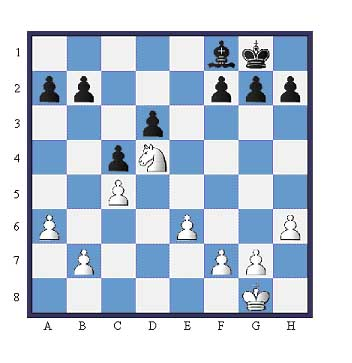
\includegraphics[height=5cm]{echiquier.jpg}$$
\end{fig}
}
\begin{ex}[Echiquier]\label{ex:echiquier}
L'échiquier de la figure \ref{fig:echiquier} ci-contre est
un ensemble de 8 lignes (numérotées de {\tt 1} à {\tt 8} sur la figure) composées
chacune de 8 cases (nommées de {\tt A} à {\tt H}).
Il peut être représenté par une liste {\tt s} de 8 listes, chacune composée de 8 éléments.
Ainsi, le roi blanc (en {\tt 8G} sur la figure) sera l'élément {\tt s[7][6]} et le 
cavalier blanc (en {\tt 4D}) sera l'élément {\tt s[3][3]} de la liste {\tt s}
en tenant compte de la convention informatique qui fait débuter à {\tt 0} les indices d'une 
liste.
\end{ex}

Le parcours d'un tableau bidimensionnel nécessite
2 boucles imbriquées : la première pour accéder aux lignes les unes après les autres,
la deuxième pour accéder aux éléments individuels de chaque ligne.

\noindent\mbox{}\hspace*{1cm}\begin{py}{6.5cm}\tt
>>> s = [[4,5],[1,2,3],[6,7,8,9]]\\
>>> for c in s: print(c) \\
... \\
\mbox{}[4, 5]\\
\mbox{}[1, 2, 3]\\
\mbox{}[6, 7, 8, 9]
\end{py}
\hfill
\begin{py}{6.5cm}\tt
>>> s[2]\\
\mbox{}[6, 7, 8, 9]\\
>>> for c in s:\\
...\ \ \ \ for e in c: print(e,end=' ')\\
...\ \ \ \ print()\\
... \\
4 5\\
1 2 3\\
6 7 8 9
\end{py}
\vspace*{2mm}

\noindent D'une manière générale, il faudra autant de boucles imbriquées qu'il y a de listes
imbriquées pour parcourir l'ensemble des éléments individuels.

\noindent\mbox{}\hspace*{1cm}\begin{py}{9cm}\tt
>>> s = [[[4,5],[1,2,3]], [[0],[10,11],[6,7,8,9]]]\\
>>> len(s)\\
2\\
>>> len(s[1])\\
3\\
>>> len(s[1][2])\\
4\\
>>> s[1][2][2]\\
8\\
>>> for c in s: print(c)\\
... \\
\mbox{}[[4, 5], [1, 2, 3]]\\
\mbox{}[[0], [10, 11], [6, 7, 8, 9]]
\end{py}
\hfill
\begin{py}{6cm}\tt
>>> for c in s:\\
...\ \ \ \ for e in c: print(e),\\
...\ \ \ \ print()\\
... \\
\mbox{}[4, 5] [1, 2, 3]\\
\mbox{}[0] [10, 11] [6, 7, 8, 9]\\
>>> for c in s:\\
...\ \ \ \ for e in c:\\
...\ \ \ \ \ \ \ \ for x in e: print(x,end=' ')\\
...\ \ \ \ print()\\
... \\
4 5 1 2 3\\
0 10 11 6 7 8 9
\end{py}
\vspace*{2mm}

Un cas particulier important de liste multidimensionnelle est la notion de matrice.
En mathématiques, les matrices servent à interpréter en termes calculatoires et 
donc opéra\-tion\-nels les résultats théoriques de l'algèbre linéaire \cite{florent77}\label{cite:florent1}.
On représente généralement une matrice $A$ sous la forme d'un tableau rectangulaire
de $n$ lignes et de $m$ colonnes :
\marginpar{\footnotesize\em
\begin{rem} Les $n$ lignes d'une matrice de dimensions $(n,m)$ ont toutes la même
longueur $m$ contrairement au cas plus général des listes multidimensionnelles qui
peuvent avoir des lignes de différentes longueurs.
\end{rem}
}
$$ A = \left(a_{ij}\right) = 
\left(
\begin{array}{rrrrr}
a_{00}     & a_{01}     & \cdots & a_{0(m-2)} & a_{0(m-1)} \\
a_{10}     & a_{11}     & \cdots & a_{1(m-2)} & a_{1(m-1)} \\
\cdots     & \cdots     & \cdots & \cdots     & \cdots \\
a_{(n-1)0} & a_{(n-1)1} & \cdots & a_{(n-1)(m-2)} & a_{(n-1)(m-1)} 
\end{array}
\right)
$$
La matrice est dite carrée quand $n=m$ et symétrique quand 
$\forall i,j\ a_{ij} = a_{ji}$.

En informatique, une matrice sera simplement représentée par un tableau bidimensionnel
comme la matrice de dimensions $(n=2,m=3)$ ci-dessous.

\noindent\mbox{}\hspace*{1cm}\begin{py}{9cm}\tt
>>> s = [[1,2,3],[4,5,6]]\\
>>> n = len(s)\\
>>> m = len(s[0])\\
>>> len(s[0]) == len(s[1])\\
True
\end{py}
\hfill
\begin{py}{6cm}\tt
>>> n\\
2\\
>>> m\\
3
\end{py}
\vspace*{2mm}


\begin{ex}[Addition de 2 matrices]\label{ex:matrices}
L'addition de 2 matrices $A$ et $B$ de mêmes dimensions $(n,m)$ donne
une nouvelle matrice $C$ de dimensions $(n,m)$ telle que $c_{ij} = a_{ij} + b_{ij}$.

\noindent\mbox{}\hspace*{1cm}\begin{py}{9cm}
\begin{verbatim}
def additionMatrice(a,b):
    n, m = len(a), len(a[0])
    s = []
    for i in range(n):
        c = []
        for j in range(m):
            c.append(a[i][j]+b[i][j])
        s.append(c)
    return s
\end{verbatim}
\end{py}
\hfill
\begin{py}{6cm}\tt
>>> a = [[1,2,3],[4,5,6]]\\
>>> b = [[-1,-2,-3],[-1,-2,-3]]\\
>>> additionMatrice(a,b)\\
\mbox{}[[0, 0, 0], [3, 3, 3]]\\
>>> additionMatrice(a,a)\\
\mbox{}[[2, 4, 6], [8, 10, 12]]
\end{py}
\end{ex}
\exo{td:matrices1}

\marginpar{\footnotesize\em
\begin{td}[Produit de matrices]\label{td:matrices1}\index[td]{opérations sur les matrices}
Définir la fonction qui calcule la matrice $C$, produit 
de 2 matrices $A$ et $B$ respectivement de dimensions $(n,r)$ et $(r,m)$.
$$c_{ij} = \sum_{k=0}^{r-1}a_{ik}\cdot b_{kj}$$
\centerline{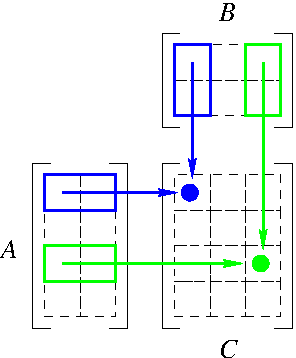
\includegraphics[width=4cm]{produit-matrices.pdf}}
\end{td}
}
Les matrices sont utilisées pour de multiples applications et servent notamment 
à représenter les coefficients des systèmes d'équations linéaires 
(voir TD \ref{td:gauss} page \pageref{td:gauss} et annexe \ref{gauss} page~\pageref{gauss}).

%-------------------------------------------------------------------------
\section{Recherche dans une séquence}\label{recherche}
%-------------------------------------------------------------------------
\marginpar{\footnotesize\em
\begin{rem} L'opération de recherche est tellement importante qu'elle est aujourd'hui 
toujours disponible dans les systèmes d'exploitation et dans les langages de programmation.
En \python, la méthode {\tt index} effectue cette recherche pour les chaînes et pour les listes.
Il est donc rarement nécessaire de la rédéfinir soi-même; nous le faisons
ici pour des raisons pédagogiques.
\end{rem}
}
En informatique, une des opérations essentielles est de retrouver une information
stockée en mémoire vive, sur un disque dur ou quelque part sur le réseau. Il suffit
pour s'en convaincre de penser au nombre de fois dans la journée  où l'on recherche
un numéro de téléphone sur son portable ou une information quelconque sur internet
à l'aide d'un moteur de recherche.

Nous nous intéresserons ici à 2 méthodes de recherche d'un élément dans une liste :
la recherche séquentielle et la recherche dichotomique.

%-------------------------------------------------------------------------
\subsection{Recherche séquentielle}\label{sub:rechercheSequentielle}
%-------------------------------------------------------------------------
La recherche séquentielle d'un élément {\tt x} dans une liste {\tt t} 
\index{recherche dans une séquence!recherche séquentielle}
consiste à comparer l'élément recherché {\tt x} successivement à tous les 
éléments de la liste {\tt t} jusqu'à trouver une correspondance.
Autrement dit, on compare l'élément recherché {\tt x} au premier élément
de la liste {\tt t}. S'ils sont identiques, on a trouvé le rang de la première 
occurence de {\tt x} dans {\tt t}; sinon, on recommence la recherche
à partir du deuxième élément. Et ainsi de suite\ldots\ On en déduit la version récursive ci-dessous
généralisée à une recherche entre deux rangs {\tt debut} et {\tt fin} de la liste {\tt t}.
Dans cette version, nous avons choisi de retourner un couple de
valeurs {\tt (ok,r)} : {\tt ok} est un booléen qui teste si la recherche est fructueuse ou non
et {\tt r} est le rang de la première occurence de l'élément recherché s'il a 
effectivement été trouvé.

\noindent\mbox{}\hspace*{1cm}\begin{py}{8cm}
\begin{verbatim}
def recherche(t,x,debut,fin):
    ok,r = False,debut
    if r > fin: ok = False
    else:
        if t[r] == x: ok = True
        else: ok,r = recherche(t,x,r+1,fin)
    return ok,r
\end{verbatim}
\end{py}
\hfill
\begin{py}{7cm}\tt
>>> s = [1,3,5,6,5,2]\\
>>> recherche(s,5,0,len(s)-1)\\
(True, 2)\\
>>> recherche(s,5,3,len(s)-1)\\
(True, 4)\\
>>> recherche(s,4,0,len(s)-1)\\
(False, 6)
\end{py}\\
\marginpar{\footnotesize\em
\begin{td}[Annuaire téléphonique]\label{td:annuaire}\index[td]{annuaire téléphonique}
On considère un annuaire téléphonique stocké sous la forme d'une liste de couples
{\tt (nom,téléphone)} (exemple : {\tt [('jean','0607080910'),('paul','0298000102')]}).
\begin{enumerate}
\item Définir une fonction qui retrouve dans un annuaire téléphonique
	le numéro de téléphone à partir du nom.
\item Définir la fonction inverse qui retrouve 
	le nom à partir du numéro de téléphone.
\end{enumerate}
\end{td}
\begin{rem}\label{rem:complexite}\index{algorithme!complexité}
On définit la complexité d'un algorithme $A$ comme une fonction $f_A(n)$ de la taille $n$ des données.
Pour analyser cette complexité, on s'attache à déterminer l'ordre de grandeur asymptotique de $f_A(n)$ :
on cherche une fonction connue qui a une rapidité de croissance voisine de celle de $f_A(n)$. On utilise pour
cela la notation mathématique $f = O(g)$, qui se lit « f est en grand O de g », et qui 
indique avec quelle rapidité une fonction « augmente » ou « diminue ». 
Ainsi $f = O(g)$ signifie que l'ordre de
grandeur asymptotique de $f$ est inférieur ou égal à celui de $g$.
$$\begin{tabular}{|l|l|}
\hline
Notation 	& Type de complexité \\
\hline
$O(1)$		& complexité constante\\
$O(\log(n))$ 	& complexité logarithmique\\
$O(n)$ 		& complexité linéaire\\
$O(n\log(n))$ 	& complexité quasi-linéaire\\
$O(n^2)$ 	& complexité quadratique\\
$O(n^3)$ 	& complexité cubique\\
$O(n^p)$ 	& complexité polynomiale\\
$O(n^{\log(n)})$ & complexité quasi-polynomiale\\
$O(2^n)$ 	& complexité exponentielle\\
$O(n!)$ 	& complexité factorielle\\
\hline
\end{tabular}$$
\end{rem}}
\exo{td:annuaire}
\vspace*{2mm}

La version itérative équivalente est donnée ci-dessous en précisant les préconditions
d'utilisation de l'algorithme.
\index[algo]{recherche séquentielle}
%\begin{lstlisting}[title={\bf Recherche séquentielle}]
%\begin{verbatim}
\begin{lstlisting}[title={\bf Recherche séquentielle}]
def rechercheSequentielle(t,x,debut,fin):
    assert type(t) is list
    assert 0 <= debut <= fin < len(t)
    ok, r = False, debut
    while r <= fin and not ok:
        if t[r] == x: ok = True
        else: r = r + 1
    return ok,r
\end{lstlisting}
%\end{verbatim}
%\end{lstlisting}

Le nombre d'itérations effectuées pour retrouver {\tt x} est égal
à la longueur $n$ de la liste {\tt t} si {\tt x} n'est pas dans la liste
et à {\tt r}, rang de la première occurence de {\tt x}, si {\tt x} est dans la liste.
Ainsi, si on définit la complexité $c$ de cet algorithme comme le nombre d'itérations
effectuées, elle est au pire égale à $n$, au mieux égale à $1$. En moyenne, on peut
démontrer (voir \cite{froidevaux} ou \cite{knuth})\label{cite:knuth1} qu'elle vaut $(1-q)\cdot n + (n+1)\cdot q/2$
si $q$ est la probabilité que {\tt x} soit dans {\tt t}, quelle que soit sa position dans la liste 
(toutes les places sont équiprobables). 
On retrouve bien
$c = n$ si $q = 0$. On a également $c = (n+1)/2$ si $q = 1$ et $c=(3n+1)/4$ si $q = 1/2$.
Dans tous les cas, l'ordre de grandeur de la complexité de la recherche séquentielle
est $n$, le nombre d'éléments dans la liste : on parle alors de complexité linéaire, 
notée $O(n)$. 
Il s'agit d'une recherche linéaire
en fonction du nombre d'éléments dans la liste : si le nombre d'éléments est multiplié par 100,
le complexité sera multipliée par 100 en moyenne, et donc le temps d'exécution de la 
recherche également.

%-------------------------------------------------------------------------
\subsection{Recherche dichotomique}\label{sub:rechercheDichotomique}
%-------------------------------------------------------------------------

Dans certains cas, la recherche d'un élément {\tt x} s'effectue dans une liste {\tt t}
triée. 
La méthode qui suit, dite recherche par dichotomie ou recherche dichotomique,
utilise pleinement le fait que les éléments de la liste sont triés.
\index{recherche dans une séquence!recherche dichotomique}

\marginpar{\footnotesize\em
\begin{rem}
Sauf mention contraire, une liste triée le sera ici selon l'ordre croissant de ses éléments.
\end{rem}
}
Le principe de la recherche dichotomique consiste à comparer {\tt x} avec l'élément
{\tt t[m]} du milieu de la liste {\tt t} :
\begin{itemize}
\item si {\tt x == t[m]}, on a trouvé une solution et la recherche s'arrête;
\item si {\tt x < t[m]}, {\tt x} ne peut se trouver que dans la moitié gauche de la liste {\tt t}
	puisque celle-ci est triée par ordre croissant; on poursuit alors la recherche
	de la même manière uniquement dans la moitié gauche de la liste;
\item si {\tt x > t[m]}, {\tt x} ne peut se trouver que dans la moitié droite de la liste {\tt t};
	on poursuit alors la recherche uniquement dans la moitié droite de la liste.
\end{itemize}
A chaque fois, on poursuit donc la recherche en diminuant de moitié le nombre d'éléments 
restant à traiter.
En suivant ce principe de recherche, on est naturellement amené à écrire une version 
récursive de l'algorithme de recherche dichotomique.

\marginpar{\footnotesize\em
\begin{td}[Recherche dichotomique]\label{td:dicho}\index[td]{recherche dichotomique}
La recherche dichotomique présentée ci-contre n'assure pas de trouver la première occurence
d'un élément {\tt x} dans une liste {\tt t} triée.\\
Modifier l'algorithme de recherche dichotomique proposé pour rechercher la
première occurence d'un élément {\tt x} dans une liste {\tt t} triée.
\end{td}
}

\noindent\mbox{}\hspace*{1cm}\begin{py}{8cm}\tt
\begin{verbatim}
def dichotomie(t,x,gauche,droite):
    ok, m = False, (gauche + droite)//2
    if gauche > droite: ok = False
    else: 
        if t[m] == x: ok = True
        elif t[m] > x: 
            ok,m = dichotomie(t,x,gauche,m-1)
        else: 
            ok,m = dichotomie(t,x,m+1,droite)
    return ok,m
\end{verbatim}
\end{py}
\hfill
\begin{py}{7cm}\tt
>>> s = [1,3,5,6,6,9]\\
>>> dichotomie(s,6,0,len(s)-1)\\
(True, 4)\\
>>> dichotomie(s,6,2,len(s)-1)\\
(True, 3)\\
>>> dichotomie(s,4,0,len(s)-1)\\
(False, 1)
\end{py}\\
\exo{td:dicho}

\marginpar{\footnotesize\em
\begin{rem}
On peut montrer (voir \cite{froidevaux} ou \cite{knuth})\label{cite:knuth2}
que la complexité de l'algorithme de recherche dichotomique est de l'ordre de
$\log(n)$ où $n$ est la longueur de la liste.
Il s'agit d'une complexité logarithmique (voir remarque \ref{rem:complexite}
page \pageref{rem:complexite}).
\end{rem}
}

La version itérative équivalente est donnée ci-dessous en précisant les préconditions
d'utilisation de l'algorithme.

\newpage
\index[algo]{recherche dichotomique}
%\begin{lstlisting}[title={\bf Recherche dichotomique}]
%\begin{verbatim}
\begin{lstlisting}[title={\bf Recherche dichotomique}]
def rechercheDichotomique(t,x,gauche,droite):
    assert type(t) is list
    assert 0 <= gauche <= droite < len(t)
    ok, m = False, (gauche + droite)/2
    while gauche <= droite and not ok:
        m = (gauche + droite)/2
        if t[m] == x: ok = True
        elif t[m] > x: droite = m - 1
        else: gauche = m + 1
    return ok,m
\end{lstlisting}
%\end{verbatim}
%\end{lstlisting}


%-------------------------------------------------------------------------
\section{Tri d'une séquence}\label{tri}
%-------------------------------------------------------------------------
Pour retrouver une information, il est souvent plus efficace que les données soient
préala\-ble\-ment triées : c'est ce que nous avons constaté avec la recherche
par dichotomie de la section précédente. Là encore, pour s'en convaincre, il suffit 
de penser à la recherche d'un mot dans un dictionnaire ou d'un nom dans un bottin.

Dans la suite, nous supposerons qu'il existe une relation d'ordre total, 
entre les éléments de la liste, notée $\leq$ et qui vérifie les propriétés 
habituelles de réflexivité, d'antisymétrie et de transitivité :
\begin{enumerate}
\item réflexivité : $x \leq x$
\item antisymétrie : $(x \leq y) \mbox{\tt\ and\ } (y \leq x) \Rightarrow x = y$
\item transitivit\'e : $(x \leq y) \mbox{\tt\ and\ } (y \leq z) \Rightarrow (x \leq z)$
\end{enumerate}
La fonction récursive {\tt enOrdre} ci-dessous teste si la liste {\tt t} est triée par
ordre croissant de ses éléments entre les rangs {\tt debut} et {\tt fin}, 
en utilisant la relation d'ordre {\tt <=} ({\tt t[debut] <= t[debut+1]}).

\noindent\mbox{}\hspace*{1cm}\begin{py}{8cm}\tt
\begin{verbatim}
def enOrdre(t,debut,fin):
    assert type(t) is list
    assert 0 <= debut <= fin < len(t)
    ok = False
    if debut == fin: ok = True
    else:
        if t[debut] <= t[debut+1]: 
            ok = enOrdre(t,debut+1,fin)
    return ok
\end{verbatim}
\end{py}
\hfill
\begin{py}{7cm}\tt
>>> s = [3,1,2,3,1]\\
>>> enOrdre(s,0,len(s)-1)\\
False\\
>>> enOrdre(s,1,3)\\
True\\
>>> enOrdre(s,1,4)\\
False
\end{py}\\
\marginpar{\footnotesize\em
\begin{td}[Liste ordonnée]\label{td:enordre}\index[td]{liste ordonnée}
Définir une version itérative de la fonction récursive {\tt enOrdre}
définie ci-contre. On appliquera la méthode de transformation décrite en
section \ref{sub:recursivite} page \pageref{methode:recursivite}.
\end{td}
}
\exo{td:enordre}

\vspace*{2mm}
      
Nous nous intéresserons ici à 3 méthodes de tri d'une liste : le tri par sélection, 
le tri par insertion et le tri rapide.

%-------------------------------------------------------------------------
\subsection{Tri par sélection}\label{sub:triSelection}
\index{tri d'une séquence!tri par sélection}
%-------------------------------------------------------------------------
\marginpar{\footnotesize\em
\begin{fig}[Tri par sélection]\label{fig:tri1}
\mbox{}\\
$\displaystyle\left\downarrow
\begin{minipage}{3.5cm}
$\begin{array}{|cccccc|}
\hline
6 & 4 & 1 & 3 & 5 & 2 \\
\hline
\end{array}$
\vspace*{1mm}

$\begin{array}{|cccccc|}
\hline
\color{blue}\bf 1 & 4 & \color{blue}\bf 6 & 3 & 5 & 2 \\
\hline
\end{array}$
\vspace*{1mm}

$\begin{array}{|cccccc|}
\hline
1 & \color{blue}\bf 2 & 6 & 3 & 5 & \color{blue}\bf 4 \\
\hline
\end{array}$
\vspace*{1mm}

$\begin{array}{|cccccc|}
\hline
1 & 2 & \color{blue}\bf 3 & \color{blue}\bf 6 & 5 & 4 \\
\hline
\end{array}$
\vspace*{1mm}

$\begin{array}{|cccccc|}
\hline
1 & 2 & 3 & \color{blue}\bf 4 & 5 & \color{blue}\bf 6 \\
\hline
\end{array}$
\vspace*{1mm}

$\begin{array}{|cccccc|}
\hline
1 & 2 & 3 & 4 & \color{blue}\bf 5 & 6 \\
\hline
\end{array}$
\vspace*{1mm}

$\begin{array}{|cccccc|}
\hline
1 & 2 & 3 & 4 & 5 & \color{blue}\bf 6 \\
\hline
\end{array}$
\end{minipage}\right.$
\hfill
\begin{minipage}{3cm}
Tri de la liste\\ {\tt [6,4,1,3,5,2]}:\\
en gras, les valeurs échan\-gées à chaque éta\-pe.
\end{minipage}
\end{fig}
}
Le tri par sélection d'une liste consiste à rechercher le minimum de la liste
à trier, de le mettre en début de liste en l'échangeant avec le premier élément
et de recommencer sur le reste de la liste (figure \ref{fig:tri1}).
La version récursive ci-dessous trie la liste {\tt t} par ordre croissant 
entre les rangs {\tt debut} et {\tt fin}; elle fait appel à la fonction {\tt minimum}
qui retourne le rang du plus petit élément de la séquence {\tt t} entre les rangs
{\tt debut} et {\tt fin}.
 
\marginpar{\footnotesize\em
\begin{td}[Tri d'un annuaire téléphonique]\label{td:tri1}\index[td]{tri d'un annuaire}
On considère un annuaire téléphonique stocké sous la forme d'une liste de couples
{\tt (nom,téléphone)} (exemple : {\tt [('paul','0607080910'),('jean','0298000102')]}).

Définir une fonction qui trie un annuaire téléphonique par ordre alphabétique des noms.
\end{td}
}
\noindent\mbox{}\hspace*{1cm}\begin{py}{8cm}\tt
\begin{verbatim}
def triSelection(t,debut,fin):
    assert type(t) is list
    assert 0 <= debut <= fin < len(t)
    if debut < fin:
        mini = minimum(t,debut,fin)
        t[debut],t[mini] = t[mini],t[debut]
        triSelection(t,debut+1,fin)
    return

>>> s = [5,4,3,2,1,0]
>>> triSelection(s,0,len(s)-1)
>>> s
[0, 1, 2, 3, 4, 5]
\end{verbatim}
\end{py}
\hfill
\begin{py}{7cm}\tt
\begin{verbatim}
def minimum(t,debut,fin):
    assert type(t) is list
    assert 0 <= debut <= fin < len(t)
    mini = debut
    for j in range(debut+1,fin+1):
        if t[j] < t[mini]: mini = j
    return mini


>>> s = [5,4,3,2,1,0]
>>> minimum(s,0,len(s)-1)
5
>>> s[minimum(s,0,len(s)-1)]
0
>>> s[minimum(s,0,2)]
3
\end{verbatim}
\end{py}\\
\exo{td:tri1}

\newpage
On en déduit la version itérative équivalente :
\index[algo]{tri par sélection}
\begin{lstlisting}[title={\bf Tri par sélection}]
def triSelection(t,debut,fin):
    assert type(t) is list
    assert 0 <= debut <= fin < len(t)
    while debut < fin:
        mini = minimum(t,debut,fin)
        t[debut],t[mini] = t[mini],t[debut]
        debut = debut + 1
    return
\end{lstlisting}

\marginpar{\footnotesize\em
\begin{td}[Complexité du tri par sélection]\label{td:tri2}\index[td]{complexité du tri par sélection}
Montrer que la complexité du tri par sélection est :
\begin{enumerate}
\item en $O(n)$ en ce qui concerne les échanges de valeurs au sein d'une liste
	de longueur $n$,
\item en $O(n^2)$ en ce qui concerne les comparaisons entre éléments de la liste.
\end{enumerate}
\end{td}
}
\exo{td:tri2}

%-------------------------------------------------------------------------
\subsection{Tri par insertion}\label{sub:triInsertion}
\index{tri d'une séquence!tri par insertion}
%-------------------------------------------------------------------------
\marginpar{\footnotesize\em
\begin{fig}[Tri par insertion]\label{fig:tri1}
\mbox{}\\
$\displaystyle\left\downarrow
\begin{minipage}{3.5cm}
$\begin{array}{|c|ccccc|}
\hline
6 & 4 & 1 & 3 & 5 & 2 \\
\hline
\end{array}$
\vspace*{1mm}

$\begin{array}{|cc|cccc|}
\hline
\color{blue}\bf 4 & 6 & 1 & 3 & 5 & 2 \\
\hline
\end{array}$
\vspace*{1mm}

$\begin{array}{|ccc|ccc|}
\hline
\color{blue}\bf 1 & 4 & 6 & 3 & 5 & 2 \\
\hline
\end{array}$
\vspace*{1mm}

$\begin{array}{|cccc|cc|}
\hline
1 & \color{blue}\bf 3 & 4 & 6 & 5 & 2 \\
\hline
\end{array}$
\vspace*{1mm}

$\begin{array}{|ccccc|c|}
\hline
1 & 3 & 4 & \color{blue}\bf 5 & 6 & 2 \\
\hline
\end{array}$
\vspace*{1mm}

$\begin{array}{|cccccc|}
\hline
1 & \color{blue}\bf 2 & 3 & 4 & 5 & 6 \\
\hline
\end{array}$
\end{minipage}\right.$
\hfill
\begin{minipage}{3cm}
Tri de la liste\\ {\tt [6,4,1,3,5,2]}:\\
en gras, les valeurs insérées dans la partie
gauche à chaque éta\-pe.
\end{minipage}
\end{fig}

\begin{rem}
Le tri par insertion correspond à la stratégie d'un joueur de cartes qui trie
son jeu.
\end{rem}
}
Dans le tri par insertion, on trie successivement les premiers éléments de la liste : à la
$i^{\grave eme}$ étape, on insère le $i^{\grave eme}$ élément à son rang parmi les $i-1$ éléments
précédents qui sont déjà triés entre eux. Dans la version récursive de la fonction 
{\tt triInsertion}, on insère l'élément {\tt t[fin]} dans la liste des éléments précédents 
déjà triée de {\tt debut} à {\tt (fin - 1)}.

\noindent\mbox{}\hspace*{1cm}\begin{py}{8cm}\tt
\begin{verbatim}
def triInsertion(t,debut,fin):
    assert type(t) is list
    assert 0 <= debut <= fin < len(t)
    if fin > debut:
        triInsertion(t,debut,fin-1)
        i = fin - 1
        x = t[fin]
        while i >= debut and t[i] > x:
            t[i+1] = t[i]
            i = i - 1
        t[i+1] = x
    return
\end{verbatim}
\end{py}
\hfill
\begin{py}{7cm}\tt
\begin{verbatim}
>>> s = [9,8,7,6,5,4]
>>> triInsertion(s,0,len(s)-1)
>>> s
[4, 5, 6, 7, 8, 9]
>>> s = [9,8,7,6,5,4]
>>> triInsertion(s,1,4)
>>> s
[9, 5, 6, 7, 8, 4]
\end{verbatim}
\end{py}

\vspace*{2mm}

La procédure précédente n'est pas récursive terminale et on ne peut donc pas utiliser
la méthode de la section \ref{sub:recursivite} page \pageref{methode:recursivite}
pour la transformer en procédure itérative.
Considérons alors une procédure récursive non terminale du type :

\noindent\mbox{}\hspace*{1cm}\begin{py}{4cm}\tt
\begin{verbatim}
def f(x):
    instruction_1
    f(g(x))
    instruction_2
    return
\end{verbatim}
\end{py}
\hfill
\begin{py}{11cm}
{\tt x} représente ici la liste des arguments de la fonction,
{\tt instruction\_1} et {\tt instruction\_2} des blocs d'instructions qui encadrent
l'appel récursif {\tt f(g(x))} et  
{\tt g(x)} une transformation des arguments de {\tt f}.
La fonction {\tt triInsertion} est bien de ce type :
{\tt x = t,debut,fin}, {\tt instruction\_1} est vide, {\tt g(x)} : {\tt t,debut,fin}
$\rightarrow$ {\tt t,debut,fin-1} et {\tt instruction\_2} regroupe toutes les instructions
qui suivent l'appel récursif.
\end{py}

\vspace*{2mm}


La méthode consiste à sauvegarder, à la fin de l'exécution de {\tt instruction\_1},
la valeur de {\tt x} sur une pile (voir section \ref{pilefile} page \pageref{pilefile}). 
Puis on exécute l'appel récursif, et on restaure la valeur de {\tt x} (on dépile {\tt x}) 
avant d'exécuter {\tt instruction\_2}.\label{recursivite:pile}
Pour un appel {\tt triInsertion(t,debut,fin)}, on va empiler successivement
{\tt fin}, {\tt fin-1}, {\tt fin-2},\ \ldots\ ,{\tt debut+1} 
(seul {\tt fin} évolue lors des appels), puis on récupèrera sur la pile les
valeurs en sens inverse {\tt debut+1}, {\tt debut+2},\ \ldots\ ,{\tt fin-2}, {\tt fin-1} et 
{\tt fin} pour chacune desquelles on exécutera la fin de la procédure. 
Une simple boucle {\tt for k in range(debut+1,fin+1)} permettra de simuler cette récupération.

La version itérative ci-dessous est équivalente à la procédure récursive. On retrouve des 
lignes 5 à 10 les instructions qui suivent l'appel récursif de la version récursive;
la boucle de la ligne 4 simule la récupération des valeurs successives de l'argument {\tt fin} 
sauvegardées avant l'appel récursif.
\marginpar{\footnotesize\em
\begin{td}[Tri par insertion]\label{td:tri3}\index[td]{tri par insertion}
Exécuter à la main l'appel\\ {\tt triInsertion([9,8,7,6,5,4],1,4)}\\ en donnant
les valeurs des variables {\tt i}, {\tt k}, {\tt x} et {\tt t} à la fin de chaque
itération de la boucle {\tt while} (ligne 7 de la version itérative de 
l'algorithme).
\end{td}
}
%\newpage
\index[algo]{tri par insertion}
%\begin{lstlisting}[title={\bf Tri par insertion}]
%\begin{verbatim}
\begin{lstlisting}[title={\bf Tri par insertion}]
def triInsertion(t,debut,fin):
    assert type(t) is list
    assert 0 <= debut <= fin < len(t)
    for k in range(debut+1,fin+1):
        i = k - 1
        x = t[k]
        while i >= debut and t[i] > x:
            t[i+1] = t[i]
            i = i - 1
        t[i+1] = x
    return
\end{lstlisting}
%\end{verbatim}
%\end{lstlisting}
\exo{td:tri3}

On peut démontrer que la complexité du tri par insertion est en $O(n^2)$
aussi bien en ce qui concerne les échanges de valeurs au sein de la liste
que les comparaisons entre éléments de la liste.

%-------------------------------------------------------------------------
\subsection{Tri rapide}\label{sub:triRapide}
\index{tri d'une séquence!tri rapide}
%-------------------------------------------------------------------------
Les complexités des tris par sélection et par insertion sont, 
soit en nombre d'échanges de valeurs, soit en nombre de comparaisons entre éléments,
quadratiques en $O(n^2)$. La méthode de tri rapide ({\em quicksort}) présentée ici 
a  une complexité quasi-linéaire en $O(n\log(n))$.

\marginpar{\footnotesize\em\vspace*{-2cm}
\begin{rem}Le tri rapide est une méthode de tri inventée par Charles Antony Richard Hoare\index{{{\sc Hoare}}} en 1961 
et basée sur le principe {\em diviser pour régner}. 
C'est en pratique un des tris sur place le plus rapide pour des données réparties aléatoirement.
\end{rem}

\begin{fig}[Partition d'une liste]\label{fig:partition}
$$\begin{tabular}{|c|c|c|}
\hline
\makebox[3cm]{$t_i \leq$ pivot} & pivot & \makebox[2cm]{$t_i >$ pivot}\\
\hline
\end{tabular}$$
La partition d'une liste est une variante du problème du drapeau hollandais dû
à l'informaticien néerlandais {\sc Edsger Wybe Dijkstra}\index{{{\sc Dijkstra}}}.
Dans sa version originale, on remplit aléatoirement un tableau avec les couleurs bleu,
blanc et rouge. Le problème consiste à trouver un algorithme qui, par des échanges successifs
de composantes, reconstitue le drapeau hollandais. L'algorithme ne doit pas utiliser de tableau
intermédiaire et ne parcourir le tableau qu'une seule fois.
\end{fig}

\begin{fig}[Tri rapide]\label{fig:tri3}
\mbox{}\\
$\displaystyle\left\downarrow
\begin{minipage}{3.5cm}
$\begin{array}{|cccccc|}
\hline
6 & 4 & 1 & 3 & 5 & 2 \\
\hline
\end{array}$
\vspace*{1mm}

$\begin{array}{|ccccc|c}
\cline{1-5}
2 & 4 & 1 & 3 & 5 & \color{blue}\bf 6\\
\cline{1-5}
\end{array}$
\vspace*{1mm}

$\begin{array}{|c|c|ccc|c}
\cline{1-1}\cline{3-5}
1 & \color{blue}\bf 2 & 4 & 3 & 5 & 6\\
\cline{1-1}\cline{3-5}
\end{array}$
\vspace*{1mm}

$\begin{array}{cc|c|c|c|c}
\cline{3-3}\cline{5-5}
1 & 2 & 3 & \color{blue}\bf 4 & 5 & 6 \\
\cline{3-3}\cline{5-5}
\end{array}$
\vspace*{1mm}

$\begin{array}{cccccc}
1 & 2 & 3 & 4 & 5 & 6 \\
\end{array}$
\end{minipage}\right.$
\hfill
\begin{minipage}{3cm}
Tri de la liste\\ {\tt [6,4,1,3,5,2]}:\\
en gras, les valeurs des pivots à chaque étape.
\end{minipage}
\end{fig}
}
Le principe du tri rapide  est le suivant : on partage la 
liste à trier en deux sous-listes telles que tous les éléments de la première 
soient inférieurs à tous les éléments de la seconde.
Pour partager la liste en deux sous-listes, on choisit un des éléments de la liste
(par exemple le premier) comme pivot. On construit alors une sous-liste
avec tous les éléments inférieurs ou égaux à ce pivot et une sous-liste avec 
tous les éléments supérieurs au pivot (figure \ref{fig:partition}).
On trie les deux sous-listes selon le même processus jusqu'à avoir des sous-listes 
réduites à un seul élément (figure \ref{fig:tri3}).

\noindent\mbox{}\hspace*{1cm}\begin{py}{8cm}\tt
\begin{verbatim}
def triRapide(t,debut,fin):
    assert type(t) is list
    assert 0 <= debut 
    assert fin <= len(t)
    if debut < fin:
        pivot = t[debut]
        place = partition(t,debut,fin,pivot)
        triRapide(t,debut,place-1)
        triRapide(t,place+1,fin)
    return
    
>>> s = [9,8,7,6,5,4]
>>> triRapide(s,0,len(s)-1)
>>> s
[4, 5, 6, 7, 8, 9]
>>> s = [9,8,7,6,5,4]
>>> triRapide(s,1,4)
>>> s
[9, 5, 6, 7, 8, 4]
\end{verbatim}
\end{py}
\hfill
\begin{py}{7cm}
\begin{verbatim}
def partition(t,debut,fin,pivot):
    p,inf,sup = debut,debut,fin;
    while p <= sup:
        if t[p] == pivot: 
            p = p + 1
        elif t[p] < pivot:
            t[inf],t[p] = t[p],t[inf]
            inf = inf + 1
            p = p + 1
        else:
            t[sup],t[p] = t[p],t[sup]
            sup = sup - 1
    if p > 0: p = p - 1
    return p


>>> s = [3,5,2,6,1,4]
>>> partition(s,0,len(s)-1,s[0]), s
(2, [1, 2, 3, 6, 5, 4])
\end{verbatim}
\end{py}

\vspace*{2mm}

\noindent Pour partitionner la liste, on a utilisé 2 compteurs {\tt inf} et {\tt sup} qui partent des
2 extrémités de la liste en évoluant l'un vers l'autre.
Le compteur de gauche {\tt inf} part du début de la liste et lorsqu'il atteint un élément 
supérieur au pivot, on arrête sa progression. De même, le compteur de droite {\tt sup}
part de la fin de la liste et s'arrête lorsqu'il atteint un élément inférieur au pivot.
On échange alors ces deux éléments ({\tt t[sup],t[inf] = t[inf],t[sup]}) puis on continue
à faire progresser les compteurs et à faire des échanges jusqu'à ce que les compteurs se
croisent.

\noindent Ainsi, le tri rapide correspond au schéma récursif suivant :

\noindent\mbox{}\hspace*{1cm}\begin{py}{4cm}\tt
\begin{verbatim}
def f(x):
    if cond:
        instructions
        f(g(x))
        f(h(x))
    return
\end{verbatim}
\end{py}
\hfill
\begin{py}{11cm}
{\tt x} représente ici la liste des arguments de la fonction,
{\tt cond} une condition portant sur {\tt x}, 
{\tt instructions} un bloc d'instructions qui précède les 2 appels
récursifs {\tt f(g(x))} et  {\tt f(h(x))}.
{\tt g(x)} et {\tt h(x)} sont des transformations des arguments de {\tt f}.
Dans le cas du tri rapide, on a {\tt g(x)} : {\tt fin = place - 1} et
{\tt h(x)} : {\tt debut = place + 1}.
\end{py}

\vspace*{2mm}

\noindent On peut supprimer le $2^{\grave eme}$ appel récursif ({\tt f(h(x))}), 
qui est terminal, selon la méthode exposée en section \ref{sub:recursivite} 
page \pageref{methode:recursivite}. Ce qui donne :

\noindent\mbox{}\hspace*{1cm}\begin{py}{4cm}\tt
\begin{verbatim}
def f(x):
    while cond:
        instructions
        f(g(x))
        x = h(x)
    return
\end{verbatim}
\end{py}
\hfill
\begin{py}{11cm}
\begin{verbatim}
def triRapide(t,debut,fin):
    assert type(t) is list
    assert 0 <= debut 
    assert fin <= len(t)
    while debut < fin:
        pivot = t[debut]
        place = partition(t,debut,fin,pivot)
        triRapide(t,debut,place-1)
        debut = place + 1
    return
\end{verbatim}
\end{py}

\vspace*{2mm}

\noindent La suppression du $1^{er}$ appel récursif ({\tt f(g(x))}) est moins immédiate 
car cet appel n'est pas terminal et la valeur des arguments {\tt x} ne varie pas de 
manière aussi prévisible que pour le tri par insertion (voir section
\ref{sub:triInsertion} page \pageref{sub:triInsertion}). 
Comme suggéré en section \ref{sub:triInsertion} page \pageref{recursivite:pile}, 
on peut utiliser une pile pour sauvegarder les contextes d'appel de la première récursivité
({\tt empiler(pile,x)}) avant de les restaurer pour la deuxième récursivité 
({\tt x = depiler(pile)}):

\noindent\mbox{}\hspace*{1cm}\begin{py}{7cm}\tt
\begin{verbatim}
def f(x):
    pile = []
    while True:
        while cond:
            instructions
            empiler(pile,x)
            x = g(x)
        if not len(pile) == 0:
            x = depiler(pile)
            x = h(x)
        else: return
    return
\end{verbatim}
\end{py}
\hfill
\begin{py}{7cm}
\begin{verbatim}
def empiler(p,x):
    assert type(p) is list
    p.append(x)
    return

def depiler(p):
    assert type(p) is list
    assert len(p) > 0
    x = p[len(p)-1]
    del p[len(p)-1]
    return x
\end{verbatim}
\end{py}

\vspace*{2mm}

\newpage
\noindent Ce qui donne la version itérative suivante pour le tri rapide :

\noindent\mbox{}\hspace*{1cm}\begin{py}{8cm}
\begin{verbatim}
def triRapide(t,debut,fin):
    assert type(t) is list
    assert 0 <= debut 
    assert fin <= len(t)
    pile = []
    while True:
        while debut < fin:
            pivot = t[debut]
            place = partition(t,debut,fin,pivot)
            empiler(pile,(debut,fin,place))
            fin = place - 1
        if not len(pile) == 0:
            (debut,fin,place) = depiler(pile)
            debut = place + 1
        else: return
    return
\end{verbatim}
\end{py}
\hfill
\begin{py}{6cm}
\begin{verbatim}
>>> s = [9,8,7,6,5,4]
>>> triRapide(s,0,len(s)-1)
>>> s
[4, 5, 6, 7, 8, 9]
>>> s = [9,8,7,6,5,4]
>>> triRapide(s,1,4)
>>> s
[9, 5, 6, 7, 8, 4]
\end{verbatim}
\end{py}

\vspace*{2mm}

\noindent A notre niveau, on retiendra cependant la version récursive, plus proche de la 
description du tri rapide :
\marginpar{\footnotesize\em
\begin{td}[Comparaison d'algorithmes (1)]\label{td:exectri1}\index[td]{comparaison d'algorithmes de tri}
Comparer les temps d'exécution des versions récursive et itérative du tri rapide pour
différentes tailles de liste.

On pourra utiliser la fonction {\tt random()} ou {\tt randint(min,max)} du module standard
{\tt random} pour générer des listes de nombres aléatoires, et la fonction {\tt time()}
du module standard {\tt time} pour mesurer le temps avant et après l'appel des
fonctions.
\end{td}
}
\index[algo]{tri rapide}
\begin{lstlisting}[title={\bf Tri rapide}]
def triRapide(t,debut,fin):
    assert type(t) is list
    assert 0 <= debut 
    assert fin <= len(t)
    if debut < fin:
        pivot = t[debut]
        place = partition(t,debut,fin,pivot)
        triRapide(t,debut,place-1)
        triRapide(t,place+1,fin)
    return
\end{lstlisting}
\exo{td:exectri1}

%-------------------------------------------------------------------------
\newpage
\setlength{\textwidth}{25cm}
\setlength{\textheight}{16cm}
\setlength{\marginparwidth}{0cm}
\setlength{\marginparsep}{0cm}
\setlength{\linewidth}{25cm}
\setlength{\oddsidemargin}{0cm}
\setlength{\evensidemargin}{0cm}
\setlength{\topmargin}{-0.75cm}

\section{Exercices complémentaires}
%-------------------------------------------------------------------------

%-------------------------------------------------------------------------
\subsection{Connaître}
%-------------------------------------------------------------------------
\begin{td}[QCM (4)]\label{td:qcmListes}(un seul item correct par question)
\index[td]{contrôle d'attention}
\em
\begin{enumerate}
\item Le type d'une variable définit 
	\begin{enumerate}
	\item l'ensemble des noms qu'elle peut prendre.
	\item le regroupement fini des données qui la composent et
		dont le nombre n'est pas fixé {\em a priori}.
	\item l'ensemble des valeurs qu'elle peut prendre et 
		l'ensemble des opérations qu'elle peut subir.
	\item le regroupement hiérarchique des données qui la composent 
	\end{enumerate}

\item Une séquence est 
	\begin{enumerate}
	\item un regroupement fini de données dont le nombre 
		n'est pas fixé {\em a priori}.
	\item une collection d'éléments, appelés « sommets », et de 
		relations entre ces sommets.
	\item une collection non ordonnée d'éléments.
	\item une suite ordonnée d'éléments
		accessibles par leur rang dans la séquence.
	\end{enumerate}

\item Parmi les exemples suivants, le seul exemple de séquence est
	\begin{enumerate}
	\item le tableau final d'un tournoi de tennis.
	\item la carte routière.
	\item la classification des espèces animales.
	\item la main au poker.
	\end{enumerate}

\item Parmi les types suivants, un seul n'est pas une variante de séquence. Lequel ?
	\begin{enumerate}
	\item le n-uplet.
	\item la chaîne de caractères.
	\item le dictionnaire.
	\item la pile.
	\end{enumerate}

\item Dans une liste 
	\begin{enumerate}
	\item tous les éléments sont du même type.
	\item les éléments peuvent avoir des types différents.
	\item les éléments ne peuvent pas être des dictionnaires.
	\item les éléments ont comme type un des types de base ({\tt bool},{\tt int},{\tt float}).
	\end{enumerate}

\item Dans la liste multidimensionnelle {\tt s = [[1,2,3,4],[5,6,7],[8,9]]} que vaut {\tt s[1][1]} ?
	\begin{enumerate}
	\item 1.
	\item 2.
	\item 5.
	\item 6.
	\end{enumerate}

\item Une pile est une séquence dans laquelle 
	\begin{enumerate}
	\item on ne peut ajouter un élément qu'à une seule extrémité 
		et ne supprimer un élément qu'à l'autre extrémité.
	\item on ne peut ajouter un élément qu'à une seule extrémité
		et en supprimer n'importe où.
	\item on ne peut ajouter et supprimer un élément
		qu'à une seule extrémité.
	\item on ne peut supprimer un élément qu'à une seule extrémité
		et en ajouter n'importe où.
	\end{enumerate}

\item Une file est une séquence dans laquelle 
	\begin{enumerate}
	\item on ne peut ajouter un élément qu'à une seule extrémité 
		et ne supprimer un élément qu'à l'autre extrémité.
	\item on ne peut ajouter un élément qu'à une seule extrémité
		et en supprimer n'importe où.
	\item on ne peut ajouter et supprimer un élément
		qu'à une seule extrémité.
	\item on ne peut supprimer un élément qu'à une seule extrémité
		et en ajouter n'importe où.
	\end{enumerate}

\item La recherche séquentielle d'un élément dans une liste consiste à 
	\begin{enumerate}
	\item rechercher le minimum de la liste et à le mettre en début de liste 
		en l'échangeant avec cet élément.
	\item rechercher le maximum de la liste et à le mettre en début de liste 
		en l'échangeant avec cet élément.
	\item comparer l'élément recherché successivement à tous les 
		éléments de la liste jusqu'à trouver une correspondance.
	\item comparer l'élément recherché avec l'élément milieu de la liste
		et poursuivre de même dans la sous-liste de droite ou 
		dans la sous-liste de gauche à l'élément milieu.
	\end{enumerate}

\item Dans le tri par insertion 
	\begin{enumerate}
	\item on partage la liste à trier en deux sous-listes telles que tous les éléments 
		de la première soient inférieurs à tous les éléments de la seconde,
		puis on trie les deux sous-listes selon le même processus jusqu'à 
		avoir des sous-listes réduites à un seul élément.
	\item on trie successivement les premiers éléments de la liste : à la $i^{\grave eme}$ étape, 
		on place le $i^{\grave eme}$ élément à son rang 
		parmi les $i-1$ éléments précédents qui sont déjà triés entre eux.
	\item on parcourt la liste en commençant par la fin, en effectuant un échange à
		chaque fois que l'on trouve deux éléments successifs qui ne sont pas 
		dans le bon ordre.
	\item on recherche le minimum de la liste à trier, on le met en début de liste 
		en l'échangeant avec le premier élément et on recommence sur le reste de la liste.
	\end{enumerate}

	{\em Parmi les 4 items de la question ci-dessus, un seul item définit le
tri par insertion, les 3 autres définissent d'autres méthodes de tri. Lesquelles ?}

\end{enumerate}
\end{td}

%-------------------------------------------------------------------------
\subsection{Comprendre}
%-------------------------------------------------------------------------
\begin{td}[Génération de séquences]\label{td:alea}
\index[td]{génération de séquences}
\em
A l'aide de la fonction {\tt randint(min,max)} du module standard {\tt random},
Définir les fonctions de génération suivantes :
\begin{enumerate}
\item {\tt liste(n)} : génère une liste de {\tt n} entiers compris entre {\tt 0} et {\tt n}.
\item {\tt nuplet(n)} : génère un n-uplet de {\tt n} entiers compris entre {\tt 0} et {\tt n}.
\item {\tt chaine(n)} : génère une chaîne de {\tt n} caractères imprimables.
\end{enumerate}
\end{td}

\begin{td}[Application d'une fonction à tous les éléments d'une liste]\label{td:foreach}
\index[td]{application d'une fonction}
\em
Définir une fonction qui applique la même fonction {\tt f} à tous les éléments d'une liste {\tt s}.

Exemples : 
\begin{tabular}[t]{l@{ , }l@{ $\rightarrow$ }l}
{\tt s = [-1,2,3,-4]}		& {\tt f = abs} & {\tt s = [1,2,3,4]}\\
{\tt s = [pi/2,pi,3*pi/2]}	& {\tt f = sin} & {\tt s = [1,0,-1]}
\end{tabular}
\end{td}


\begin{td}[Que fait cette procédure ?]\label{td:trishell}
\index[td]{que fait cette procédure ?}
\em
On considère la procédure {\tt f} ci-dessous.

\noindent\mbox{}\hspace*{1cm}\begin{py}{7cm}\tt
\begin{verbatim}
def f(t,debut,fin):
    m = (debut + fin)//2
    while m > 0:
        for i in range(m,fin+1):
            j = i - m
            while j >= debut:
                print(m,i,j,t)
                if t[j] > t[j+m]:
                    t[j],t[j+m] = t[j+m],t[j]
                    j = j - m
                else: j = debut-1
        m = m//2
    return 
\end{verbatim}
\end{py}

\vspace*{2mm}

\begin{enumerate}
\item Tracer l'exécution {\em à la main} de l'appel {\tt f([4,2,1,2,3,5],0,5)}.
\item Que fait cette procédure ?
\end{enumerate}

\end{td}

%-------------------------------------------------------------------------
\subsection{Appliquer}
%-------------------------------------------------------------------------
\begin{td}[Codes ASCII et chaînes de caractères]\label{td:asciichaines}\index[td]{codes ASCII et chaînes de caractères}
\em
\begin{enumerate}
\item Ecrire un algorithme qui fournit le tableau des codes ASCII
        (annexe \ref{ascii} page \pageref{ascii}) associé
        à une chaîne (exemple : {\tt 'bon'} $\rightarrow$ {\tt [98, 111, 110]}).
\item Ecrire un algorithme qui donne la chaîne de caractères associée à un tableau de codes
        ASCII (exemple : {\tt [98, 111, 110]} $\rightarrow$ {\tt 'bon'}).
\end{enumerate}
\end{td}

\begin{td}[Opérations sur les matrices]\label{td:matrices2}\index[td]{opérations sur les matrices}
\em
\begin{enumerate}
\item Définir une fonction qui teste si une liste {\tt m} est une matrice.
\item Définir une fonction qui teste si une matrice {\tt m} est une matrice carrée.
\item Définir une fonction qui teste si une matrice {\tt m} est une matrice symétrique.
\item Définir une fonction qui teste si une matrice {\tt m} est une matrice diagonale.
\item Définir une fonction qui multiplie une matrice {\tt m} par un scalaire {\tt x}.
\item Définir une fonction qui détermine la transposée d'une matrice {\tt m}.
\end{enumerate}
\end{td}

%-------------------------------------------------------------------------
\subsection{Analyser}
%-------------------------------------------------------------------------
\begin{td}[Recherche d'un motif]\label{td:motif}\index{recherche dans une séquence!recherche d'un motif}
\index[td]{recherche d'un motif}
\em
Définir un algorithme qui recherche la première occurence d'une séquence {\tt m}
au sein d'une autre séquence {\tt t}.
\end{td}

\begin{td}[Recherche de toutes les occurences]\label{td:occurs}
\index[td]{recherche de toutes les occurences}
\em
Définir une fonction qui retourne la liste des rangs de toutes les occurences
d'un élément {\tt x} dans une liste {\tt t}.
\end{td}

\begin{td}[Tri bulles]\label{td:bulles}\index{tri d'une séquence!tri bulles}
\index[td]{tri bulles}
\em
Dans le tri bulles, on parcourt la liste en commençant par la fin, en effectuant un échange à
chaque fois que l'on trouve deux éléments successifs qui ne sont pas dans le bon ordre.

\noindent Définir une fonction qui trie une liste selon la méthode du tri bulles.
\end{td}

\begin{td}[Méthode d'élimination de {\sc Gauss}]\label{td:gauss}\index[td]{méthode d'élimination de {{\sc Gauss}}}
\em
L'objectif est ici de 
résoudre dans $\mathbb{R}$ un système de $n$ équations linéaires
à $n$ inconnues, homogènes ou non homogènes, du type $A\cdot x = b$ :
$$\left\{
\begin{array}{r@{\ +\ }r@{\ +\ }r@{\ +\ }r@{\ =\ }r}
a_{00}x_0     & a_{01}x_1     & \cdots & a_{0(n-1)}x_{(n-1)}     & b_0      \\
a_{10}x_0     & a_{11}x_1     & \cdots & a_{1(n-1)}x_{(n-1)}     & b_1      \\
\cdots        & \cdots        & \cdots & \cdots                  & \cdots   \\
a_{(n-1)0}x_0 & a_{(n-1)1}x_1 & \cdots & a_{(n-1)(n-1)}x_{(n-1)} & b_{(n-1)}
\end{array}
\right.$$
Définir une fonction {\tt solve(a,b)} qui retourne le vecteur {\tt x}
solution du système linéaire $A\cdot x = b$ selon la méthode d'élimination de 
{\sc Gauss} décrite en section \ref{gauss} page \pageref{gauss}.
\end{td}

%-------------------------------------------------------------------------
\subsection{Evaluer}
%-------------------------------------------------------------------------
\begin{td}[Comparaison d'algorithmes de recherche.]\label{td:exectri2}\index[td]{comparaison d'algorithmes de recherche}
\em
Comparer les temps d'exécution des versions récursive et itérative des
2 méthodes de recherche développées dans le cours (section \ref{recherche}).

On pourra utiliser la fonction {\tt random()} ou {\tt randint(min,max)} du module standard
{\tt random} pour générer des listes de nombres aléatoires, et la fonction {\tt time()}
du module standard {\tt time} pour mesurer le temps avant et après l'appel des
fonctions.
\end{td}

\begin{td}[Comparaison d'algorithmes de tri]\label{td:exectri3}\index[td]{comparaison d'algorithmes de tri}
\em
Comparer les temps d'exécution des différentes versions récursives et itératives des
3 méthodes de tri développées dans le cours (section \ref{tri}).

On pourra utiliser la fonction {\tt random()} ou {\tt randint(min,max)} du module standard
{\tt random} pour générer des listes de nombres aléatoires, et la fonction {\tt time()}
du module standard {\tt time} pour mesurer le temps avant et après l'appel des
fonctions.
\end{td}

%-------------------------------------------------------------------------
\subsection{Solutions des exercices}\label{sub:solutionsListes}
%-------------------------------------------------------------------------
\begin{description}
\item[TD \ref{td:qcmListes} :] QCM (4).\\
	Les bonnes réponses sont extraites directement
	du texte de ce chapitre : \\
	1c, 2d, 3d, 4c, 5b, 6d, 7c, 8a, 9c, 10b

\item[TD \ref{td:alea} :] Génération de séquences.
\begin{enumerate}
\item Génération de listes d'entiers.

\begin{py}{6cm}
\begin{verbatim}
def liste(n):
    assert type(n) is int and n >= 0
    t = []
    for i in range(n):
        t.append(randint(0,n))
    return t
\end{verbatim}
\end{py}
\hfill
\begin{py}{6cm}
\begin{verbatim}
>>> liste(0)
[]
>>> liste(10)
[6, 7, 9, 8, 5, 4, 9, 1, 8, 9]
\end{verbatim}
\end{py}
\vspace*{2mm}

%\newpage
\item Génération de n-uplets d'entiers.

\begin{py}{6cm}
\begin{verbatim}
def nuplet(n):
    assert type(n) is int and n >= 0
    t = ()
    for i in range(n):
        t = t + (randint(0,n),)
    return t
\end{verbatim}
\end{py}
\hfill
\begin{py}{6cm}
\begin{verbatim}
>>> nuplet(0)
()
>>> nuplet(10)
(6, 2, 3, 10, 9, 3, 4, 1, 3, 4)
\end{verbatim}
\end{py}
\vspace*{2mm}

\item Génération de chaînes de caractères.

\begin{py}{6cm}
\begin{verbatim}
def chaine(n):
    assert type(n) is int and n >= 0
    t = ''
    for i in range(n):
        t = t + chr(randint(32,127)
    return t
\end{verbatim}
\end{py}
\hfill
\begin{py}{6cm}
\begin{verbatim}
>>> chaine(0)
''
>>> chaine(10)
'kN K,-`Phe'
\end{verbatim}
\end{py}
\vspace*{2mm}

\end{enumerate}

\item[TD \ref{td:foreach} :] Application d'une fonction à tous les éléments d'une liste.

\begin{py}{6cm}
\begin{verbatim}
def application(f,t):
    assert type(t) is list
    for i in range(len(t)): t[i] = f(t[i])
    return t
\end{verbatim}
\end{py}
\hfill
\begin{py}{6cm}
\begin{verbatim}
s = [pi/2,pi,3*pi/2]
>>> application(sin,s)
[1.0, 1.2246063538223773e-16, -1.0]
\end{verbatim}
La fonction prédéfinie {\tt map(f,t)} fait la même chose.
\begin{verbatim}
>>> s = [pi/2,pi,3*pi/2]
>>> map(sin,s)
[1.0, 1.2246063538223773e-16, -1.0]
\end{verbatim}
\end{py}
\vspace*{2mm}

\item[TD \ref{td:trishell} :] Que fait cette procédure ? 

\begin{py}{4cm}
\begin{verbatim}
>>> f([4,2,1,2,3,5],0,5)
2 2 0 [4, 2, 1, 2, 3, 5]
2 3 1 [1, 2, 4, 2, 3, 5]
2 4 2 [1, 2, 4, 2, 3, 5]
2 4 0 [1, 2, 3, 2, 4, 5]
2 5 3 [1, 2, 3, 2, 4, 5]
1 1 0 [1, 2, 3, 2, 4, 5]
1 2 1 [1, 2, 3, 2, 4, 5]
1 3 2 [1, 2, 3, 2, 4, 5]
1 3 1 [1, 2, 2, 3, 4, 5]
1 4 3 [1, 2, 2, 3, 4, 5]
1 5 4 [1, 2, 2, 3, 4, 5]
\end{verbatim}
\end{py}
\hfill
\begin{minipage}[t]{9cm}
\index{tri d'une séquence!tri shell}
Cette procédure trie une liste selon la méthode du tri par incrément décroissant (tri shell).
Au premier passage, on considère des sous-listes d'éléments distants de {\tt m = (debut+fin)/2}
que l'on trie séparément. Au deuxième passage, on considère des sous-listes d'éléments distants 
de {\tt m/2} que l'on trie séparément, et ainsi de suite. A chaque passage, l'incrément {\tt m} est
divisé par 2 et toutes les sous-listes sont triées. Le tri s'arrête quand l'incrément est nul.
\end{minipage}
\vspace*{2mm}

\item[TD \ref{td:asciichaines} :] Codes ASCII et chaînes de caractères.
\begin{enumerate}
\item Chaîne $\rightarrow$ codes ASCII
	
\begin{py}{6cm}
\begin{verbatim}
def codeASCII(s):
    code = []
    for i in range(len(s)):
        code.append(ord(s[i]))
    return code
\end{verbatim}
\end{py}
\hfill
\begin{py}{6cm}
\begin{verbatim}
>>> codeASCII('bon')
[98, 111, 110]
\end{verbatim}
\end{py}
\vspace*{2mm}

\item Codes ASCII $\rightarrow$ chaîne

\begin{py}{6cm}
\begin{verbatim}
def decodeASCII(code):
    s = ''
    for i in range(len(code)):
        s = s + chr(code[i])
    return s
\end{verbatim}
\end{py}
\hfill
\begin{py}{6cm}
\begin{verbatim}
>>> decodeASCII([98, 111, 110])
'bon'
\end{verbatim}
\end{py}
\vspace*{2mm}

\end{enumerate}

\item[TD \ref{td:matrices2} :] Opérations sur les matrices.\\
\begin{enumerate}
\item Matrice.

\begin{py}{6cm}
\begin{verbatim}
def matrice(t):
    ok = True
    if type(t) is not list or t == []:
        ok = False
    elif type(t[0]) is not list: 
        ok = False
    else:
        i, n, m = 1, len(t), len(t[0])
        while i < n and ok == True:
            if type(t[i]) is not list:
                ok = False
            elif len(t[i]) != m: 
                ok = False
            i = i + 1
    return ok
\end{verbatim}
\end{py}
\hfill
\begin{py}{6cm}
\begin{verbatim}
>>> matrice(5)
False
>>> matrice([])
False
>>> matrice([5])
False
>>> matrice([[5]])
True
>>> matrice([[5,6],
             [7]])
False
>>> matrice([[5,6,7],
             [8,9]])
False
>>> matrice([[5,6,7],
             [8,9,3]])
True
\end{verbatim}
\end{py}
\vspace*{2mm}

\newpage
\item Matrice carrée.

\begin{py}{6cm}
\begin{verbatim}
def matriceCarree(t):
    assert matrice(t)
    if len(t) > 0 and len(t[0]) == len(t):
        ok = True
    else: ok = False
    return ok
\end{verbatim}
\end{py}
\hfill
\begin{py}{6cm}
\begin{verbatim}
>>> matriceCarree([[4,5,6],
                   [7,8,9]])
False
>>> matriceCarree([[5,6],
                   [8,9]])
True
>>> matriceCarree([[]])
False
\end{verbatim}
\end{py}
\vspace*{2mm}

\item Matrice symétrique.

\begin{py}{6cm}
\begin{verbatim}
def matriceSymetrique(t):
    assert matriceCarree(t)
    ok,i = True,0
    while i < len(t) and ok == True:
        j = i + 1
        while j < len(t[0]) and ok == True:
            if t[i][j] != t[j][i]: 
                ok = False
            else: j = j + 1
        i = i + 1
    return ok
\end{verbatim}
\end{py}
\hfill
\begin{py}{6cm}
\begin{verbatim}
>>> matriceSymetrique([[5,6],
                       [8,9]])
False
>>> matriceSymetrique([[5,6],
                       [6,9]])
True
>>> matriceSymetrique([[5,6,7],
                       [6,8,9],
                       [7,9,3]])
True
\end{verbatim}
\end{py}
\vspace*{2mm}

\item Matrice diagonale.

\begin{py}{6cm}
\begin{verbatim}
def matriceDiagonale(t):
    assert matriceCarree(t)
    ok,i = True,0
    while i < len(t) and ok == True:
        j = 0
        while j < len(t[0]) and ok == True:
            if i != j and t[i][j] != 0:
                ok = False
            else: j = j + 1
        i = i + 1
    return ok
\end{verbatim}
\end{py}
\hfill
\begin{py}{6cm}
\begin{verbatim}
>>> matriceDiagonale([[5,6],
                      [8,9]])
False
>>> matriceDiagonale([[5,0],
                      [0,9]])
True
>>> matriceDiagonale([[5,0,0],
                      [0,0,0],
                      [0,0,3]])
True
\end{verbatim}
\end{py}
\vspace*{2mm}

\newpage
\item Multiplication d'une matrice par un scalaire.

\begin{py}{6cm}
\begin{verbatim}
def multiplicationScalaire(t,x):
    assert matrice(m)
    assert type(x) is int or type(x) is float
    for i in range(len(t)):
        for j in range(len(t[0])):
            t[i][j] = x*t[i][j]
    return
\end{verbatim}
\end{py}
\hfill
\begin{py}{6cm}
\begin{verbatim}
>>> multiplicationScalaire([[5,6],
                            [2,7]],3)
[[15, 18], [6, 21]]
\end{verbatim}
\end{py}
\vspace*{2mm}

\item Transposée d'une matrice.

\begin{py}{6cm}
\begin{verbatim}
def transposee(t):
    assert matrice(t)
    s = []
    for j in range(len(t[0])):
        s.append([])
        for i in range(len(t)):
            s[j].append(t[i][j])
    return s
\end{verbatim}
\end{py}
\hfill
\begin{py}{6cm}
\begin{verbatim}
>>> transposee([[1,2],[4,5]])
[[1, 4], [2, 5]]
>>> transposee([[1,2,3],[4,5,6]])
[[1, 4], [2, 5], [3, 6]]
\end{verbatim}
\end{py}
\vspace*{2mm}

\end{enumerate}

\item[TD \ref{td:motif} :] Recherche d'un motif.\\

\begin{py}{6cm}
\begin{verbatim}
def motif(t,m,debut,fin):
    assert type(t) is list
    assert type(m) is list
    assert 0 <= debut <= fin < len(t)
    i,ok = debut,False
    while i + len(m) - 1 <= fin and not ok:
        if t[i:i+len(m)] == m and m != []:
            ok = True
        else: i = i + 1
    return ok,i
\end{verbatim}
\end{py}
\hfill
\begin{py}{6cm}
\begin{verbatim}
>>> motif([1,2,3,2,3,4],[2,4],0,5)
(False, 5)
>>> motif([1,2,3,2,3,4],[2,3],0,5)
(True, 1)
>>> motif([1,2,3,2,3,4],[2,3],2,5)
(True, 3)
>>> motif([1,2,3,2,3,4],[2,3,4],0,5)
(True, 3)
\end{verbatim}
\end{py}
\vspace*{2mm}

\item[TD \ref{td:occurs} :] Recherche de toutes les occurences.

\begin{py}{6cm}
\begin{verbatim}
def rechercheTout(t,x):
    assert type(t) is list
    occurs = []
    for i in range(len(t)):
        if t[i] == x: occurs.append(i)
    return occurs
\end{verbatim}
\end{py}
\hfill
\begin{py}{6cm}
\begin{verbatim}
>>> rechercheTout([1,2,1,5,1],1)
[0, 2, 4]
>>> rechercheTout([1,2,1,5,1],2)
[1]
>>> rechercheTout([1,2,1,5,1],3)
[]
\end{verbatim}
\end{py}
\vspace*{2mm}

\newpage
\item[TD \ref{td:bulles} :] Tri bulles.

\begin{py}{6cm}
\begin{verbatim}
def triBulles(t,debut,fin):
    assert type(t) is list
    assert 0 <= debut <= fin < len(t)
    while debut < fin:
        for j in range(fin,debut,-1):
            if t[j] < t[j-1]: 
                t[j],t[j-1] = t[j-1],t[j]
        debut = debut + 1
    return t
\end{verbatim}
\end{py}
\hfill
\begin{py}{6cm}
\begin{verbatim}
>>> s = [9,8,7,6,5,4]
>>> triBulles(s,0,len(s)-1)
[4, 5, 6, 7, 8, 9]
>>> s = [9,8,7,6,5,4]
>>> triBulles(s,1,4)
[9, 5, 6, 7, 8, 4]
\end{verbatim}
\end{py}
\vspace*{2mm}


\item[TD \ref{td:gauss} :] Méthode d'élimination de {\sc Gauss}.

\begin{py}{6cm}
\begin{verbatim}
def solve(a,b):
    assert matriceCarree(a) 
    assert type(b) is list
    assert len(a) == len(b)
    if triangularisation(a,b) == True:
        x = backsubstitutions(a,b)
    else: x = []
    return x

>>> a, b = [[4]], [1]
>>> solve(a,b)
[0.25]
>>> a, b = [[1,1],[1,-1]], [1,0]
>>> solve(a,b)
[0.5, 0.5]
>>> a = [[2,-1,2],[1,10,-3],[-1,2,1]]
>>> b = [2,5,-3]
>>> solve(a,b)
[2.0, 0.0, -1.0]
\end{verbatim}
\end{py}
\hfill
\begin{py}{6cm}
\begin{verbatim}
>>> a = [[ 1,  0, 0, -1,  1, 0],
         [ 1,  1, 0,  0,  0,-1],
         [ 0,  1,-1,  0, -1, 0],
         [10,-10, 0,  0,-10, 0],
         [ 0,  0, 5,-20,-10, 0],
         [ 0, 10, 5,  0,  0,10]]
>>> b = [0,0,0,0, 0,12]
>>> solve(a,b)
[0.25945945945945936, 
 0.35675675675675667, 
 0.45405405405405402, 
 0.16216216216216217, 
-0.097297297297297303, 
 0.61621621621621636]
\end{verbatim}
\end{py}
\vspace*{2mm}

\begin{py}{14cm}
\begin{verbatim}
>>> a, b = [[10,7,8,7],[7,5,6,5],[8,6,10,9],[7,5,9,10]], [32,23,33,31]
>>> solve(a,b)
[1.0000000000000102, 0.99999999999998335, 1.000000000000004, 0.99999999999999778]
>>> a = [[10,7,8.1,7.2],[7.08,5.04,6,5],[8,5.98,9.89,9],[6.99,4.99,9,9.98]]
>>> solve(a,b)
[28714.563366527444, -47681.976061485781, 12326.759748689999, -7387.0215554531824]
>>> a = [[10,7,8,7],[7,5,6,5],[8,6,10,9],[7,5,9,10]], [32.01,22.99,33.01,30.99]
>>> solve(a,b)
[1.8199999999999306, -0.35999999999988425, 1.3499999999999692, 0.79000000000001847]
\end{verbatim}
\end{py}

\newpage

\begin{py}{6cm}
\begin{verbatim}
def pivot(a,i0):
    maxi = fabs(a[i0][i0])
    r = i0
    for i in range(i0+1,len(a)):
      if fabs(a[i][i0]) > maxi:
          maxi = fabs(a[i][i0])
          r = i
    return r
\end{verbatim}
\end{py}
\hfill
\begin{py}{6cm}
\begin{verbatim}
def substractRows(a,b,k,i):
    q = 1.*a[k][i]/a[i][i]
    a[k][i] = 0
    b[k] = b[k] - q*b[i]
    for j in range(i+1,len(a)):
        a[k][j] = a[k][j] - q*a[i][j]
    return 
\end{verbatim}
\end{py}
\vspace*{2mm}

\begin{py}{6cm}
\begin{verbatim}
def triangularisation(a,b):
   ok = True; i = 0
   while i < len(a) and ok == True:
      p = pivot(a,i)
      if i != p:
         a[i],a[p] = a[p],a[i]
         b[i],b[p] = b[p],b[i]
      if a[i][i] == 0: ok = False
      else:
         for k in range(i+1,len(a)):
            substractRows(a,b,k,i)
      i = i + 1
   return ok
\end{verbatim}
\end{py}
\hfill
\begin{py}{6cm}
\begin{verbatim}
def backsubstitutions(a,b):
    n = len(a); x = []
    for k in range(n): x.append(0)
    
    x[n-1] = 1.*b[n-1]/a[n-1][n-1]
    for i in range(n-2,-1,-1): 
        x[i] = b[i]
        for j in range(i+1,n):
            x[i] = x[i] - a[i][j]*x[j]
        x[i] = 1.*x[i]/a[i][i]
    return x
\end{verbatim}
\end{py}
\vspace*{2mm}

\item[TD \ref{td:exectri2} :] Comparaison d'algorithmes de recherche.

\begin{py}{4cm}
\begin{verbatim}
def mesureRecherche(f,t,x):
    t0 = time()
    f(tmp,x,0,len(t)-1)
    dt = time() - t0
    return dt
\end{verbatim}
\end{py}
\hfill
\begin{py}{9cm}
\begin{verbatim}
>>> s = liste(1000)
>>> x = s[len(s)-1]
>>> mesureRecherche(rechercheSequentielle,s,x)
0.00062489509582519531
>>> s = liste(100000)
>>> x = s[len(s)-1]
>>> mesureRecherche(rechercheSequentielle,s,x)
0.046545028686523438
\end{verbatim}
\end{py}
\vspace*{2mm}

%\newpage
\item[TD \ref{td:exectri3} :] Comparaison d'algorithmes de tri.

\begin{py}{4cm}
\begin{verbatim}
def mesureTri(f,t):
    tmp = [x for x in t]
    t0 = time()
    f(tmp,0,len(t)-1)
    dt = time() - t0
    return dt
\end{verbatim}
\end{py}
\hfill
\begin{py}{9cm}
\begin{verbatim}
>>> s = liste(10000)
>>> mesureTri(triSelection,s)
23.040315866470337
>>> mesureTri(triInsertion,s)
22.086866855621338
>>> mesureTri(triRapide,s)
0.24324798583984375
\end{verbatim}
\end{py}
\vspace*{2mm}

\end{description}

%-------------------------------------------------------------------------
\newpage
\setlength{\textwidth}{16cm}
\setlength{\linewidth}{16cm}
\setlength{\textheight}{16cm}
\setlength{\marginparwidth}{8cm}
\setlength{\marginparsep}{1cm}
\setlength{\oddsidemargin}{0cm}
\setlength{\evensidemargin}{+8cm}
\setlength{\topmargin}{-0.75cm}

\section{Annexes}
%-------------------------------------------------------------------------

%-------------------------------------------------------------------------
\subsection{Type abstrait de données}\label{tad:sequence}\index{type abstrait de données}
%-------------------------------------------------------------------------
Nous nous intéressons ici à une description plus formelle du type abstrait de données {\tt Sequence} selon un formalisme
logique inspiré de \cite{manna}. 
On notera $\Bbb B$ l'ensemble des booléens ($\{0,1\}$),
$\Bbb E$ l'ensemble des éléments, $\Bbb S$ l'ensemble des séquences, $\Bbb F$ l'ensemble
des fonctions $\Bbb E \rightarrow \Bbb E$ et $\Bbb P$ l'ensemble des fonctions
$\Bbb E \rightarrow \Bbb B$.
Le vocabulaire initial de la th\'eorie des séquences comprend alors:
\begin{itemize}
\item une constante {\tt []} qui représente la séquence vide (on notera $\Bbb S^* = \Bbb S - \{\mbox{\tt []}\}$);
\item un opérateur $x \circ s$ qui traduit l'insertion d'un élément $x\in \Bbb E$ en tête
	de la séquence $s \in \Bbb S$.
\end{itemize}
Dans ce cadre, la définition axiomatique des séquences repose sur les 2 axiomes suivants :
\begin{enumerate}
\item {\tt []} est une séquence : $\mbox{\tt []} \in \Bbb S $,
\item $x \circ s$ est une séquence : $\forall x \in {\Bbb E},\ \forall s \in {\Bbb S},\ x \circ s \in {\Bbb S}$.
\end{enumerate}

Pour chaque opération considérée, nous indiquerons sa signature, sa définition axiomatique 
(souvent récursive) et son équivalent {\color{blue}\python}.
\begin{itemize}
\item ${\rm head}(s)$ : tête (premier élément) d'une séquence\\
{\begin{tabular}{p{1cm}@{ : }p{2cm}@{ , }p{6.75cm}p{4.5cm}}
head & $\Bbb S^* \rightarrow \Bbb E$ 	& $x = {\rm head}(x \circ s)$				& \color{blue}\tt s[0]
\end{tabular}}

\item ${\rm tail}(s)$ : queue d'une séquence (la séquence sans son premier élément)\\
{\begin{tabular}{p{1cm}@{ : }p{2cm}@{ , }p{6.75cm}p{4.5cm}}
tail & $\Bbb S^* \rightarrow \Bbb E$	& $s = {\rm tail}(x \circ s)$				& \color{blue}\tt s[1\char`:len(s)]
\end{tabular}}

\item $x \mbox{\rm\ in\ s}$ : appartenance d'un élément à une séquence\\
{\begin{tabular}{p{1cm}@{ : }p{2cm}@{ , }p{6.75cm}p{4.5cm}}
in & $\Bbb E \times \Bbb S \rightarrow \Bbb B$	 & $\displaystyle\left|\begin{array}{l}x = {\rm head}(s)\\ 
                                                                                              x \mbox{\rm\ in\ } {\rm tail}(s)\end{array}\right.$ & \color{blue}\tt x in s
\end{tabular}}

\item ${\rm len}(s)$ : longueur d'une séquence (nombre d'éléments)\\
{\begin{tabular}{p{1cm}@{ : }p{2cm}@{ , }p{6.75cm}p{4.5cm}}
len & $\Bbb S \rightarrow \Bbb N$	& $\displaystyle\left|\begin{array}{l}{\rm len}(\mbox{\tt []}) = 0\\ 
                                                                                              {\rm len}(x \circ s) = {\rm len}(s) + 1\end{array}\right.$ & \color{blue}\tt len(s)
\end{tabular}}

\item ${\rm concat}(s_1,s_2)$ (ou $s_1+s_2$) : concaténation de deux séquences\\
{\begin{tabular}{p{1cm}@{ : }p{2cm}@{ , }p{6.75cm}p{4.5cm}}
concat & $\Bbb S \times \Bbb S \rightarrow \Bbb S$	& $\displaystyle\left|\begin{array}{l}\mbox{\tt []} + s = s\\ 
                                                                                              s_3 = (x \circ s_1) + s_2 = x \circ (s_1 + s_2)\end{array}\right.$ & \color{blue}\tt s1 + s2
\end{tabular}}

\item ${\rm ith}(s,i)$ (ou $s_i$) : $i^{\grave eme}$ élément de la séquence\\
{\begin{tabular}{p{1cm}@{ : }p{2cm}@{ , }p{6.75cm}p{4.5cm}}
ith & $\Bbb S^* \times \Bbb N \rightarrow \Bbb E$      & $\displaystyle\left|\begin{array}{l}(x \circ s)_0 = x\\ 
                                                                                              (x \circ s)_i = s_{i-1}\ \ \mbox{\footnotesize\ $0 < i \leq {\rm len}(s)$}\end{array}\right.$ & \color{blue}\tt s[i]
\end{tabular}}

\item ${\rm foreach}(f,s)$ : application d'une fonction à tous les éléments d'une séquence\\
{\begin{tabular}{p{1cm}@{ : }p{2cm}@{ , }p{6.75cm}p{4.5cm}}
foreach & $\Bbb F \times \Bbb S \rightarrow \Bbb S$	& $\displaystyle\left|\begin{array}{l}{\rm foreach}(f,\mbox{\tt []}) = \mbox{\tt []}\\ 
                                                                                              {\rm foreach}(f,x\circ s) = f(x)\circ {\rm foreach}(f,s)\end{array}\right.$ & \color{blue}\tt [f(x) for x in s]
\end{tabular}}

\marginpar{\footnotesize\em
\begin{fig}[Codes des caractères de contrôle]\label{fig:ascii}
$$\begin{tabular}{lll}
code & caractère & signification \\
\hline
0 & NUL & \em Null\\
1 & SOH & \em Start of heading\\
2 & STX & \em Start of text\\
3 & ETX & \em End of text\\
4 & EOT & \em End of transmission\\
5 & ENQ & \em Enquiry\\
6 & ACK & \em Acknowledge\\
7 & BEL & \em Bell\\
8 & BS  & \em Backspace\\
9 & TAB & \em Horizontal tabulation\\
10 & LF & \em Line Feed\\
11& VT  & \em Vertical tabulation\\
12& FF  & \em Form feed\\
13& CR  & \em Carriage return\\
14& SO  & \em Shift out\\
15& SI  & \em Shift in\\
16& DLE & \em Data link escape\\
17& DC1 & \em Device control 1\\
18& DC2 & \em Device control 2\\
19& DC3 & \em Device control 3\\
20& DC4 & \em Device control 4\\
21& NAK & \em Negative acknowledgement\\
22& SYN & \em Synchronous idle\\
23& ETB & \em End of transmission block\\
24& CAN & \em Cancel\\    
25& EM  & \em End of medium\\
26& SUB & \em Substitute\\
27& ESC & \em Escape\\
28& FS  & \em File separator\\
29& GS  & \em Group separator\\
30& RS  & \em Record separator\\
31& US  & \em Unit separator\\
\end{tabular}$$
\end{fig}}

\item ${\rm collect}(p,s)$ : sélection sous condition des éléments d'une séquence\\
{\begin{tabular}{p{1cm}@{ : }p{2cm}@{ , }p{6.75cm}p{4.5cm}}
collect & $\Bbb P \times \Bbb S \rightarrow \Bbb S$	& $\displaystyle\left|\begin{array}{l}{\rm collect}(p,\mbox{\tt []}) = \mbox{\tt []}\\ 
							                                      {\rm collect}(p,x\circ s) = x\circ {\rm collect}(p,s) \mbox{ si } p(x)\\
											      {\rm collect}(p,x\circ s) = {\rm collect}(p,s) \mbox{ si } \neg p(x)\end{array}\right.$ & 
											      \color{blue}\tt [x for x in s if p(x)]
\end{tabular}}
\end{itemize}


%-----------------------------------------------------------------------------
\subsection{Codes ASCII}\label{ascii}\index{codes ASCII}
%-----------------------------------------------------------------------------
L'ordinateur stocke toutes les données sous forme numérique
(ensemble de bits). En particulier, les caractères ont un équivalent numérique : 
le code ASCII ({\em American Standard Code for Information Interchange}). 
Le code ASCII de base code les caractères sur 7 bits (128 caractères, de 0 à 127).
\begin{itemize}
\item Les codes 0 à 31 sont des caractères de contrôle (figure \ref{fig:ascii}).
\item Les codes 32 à 47, de 58 à 64, de 91 à 96 et de 123 à 126 
	sont des symboles de ponctuation.
{\footnotesize\tt$$\begin{tabular}{|cccccccccccccccc|}
\hline
32 & 33 & 34 & 35 & 36 & 37 & 38 & 39 & 40 & 41 & 42 & 43 & 44 & 45 & 46 & 47 \\
   & !  & " 	& \# & \$ & \% & \& & '  & (  &	)  & * 	& +  & ,  & -  & .  & / \\
\hline
\end{tabular}$$}
{\footnotesize\tt$$\begin{tabular}{|ccccccc|}
\hline
58 & 59 & 60 & 61 & 62 & 63 & 64 \\
:  & ;  & <  & =  & >  & ?  & @	\\
\hline
\end{tabular}\hspace*{2mm}
\begin{tabular}{|cccccc|}
\hline
91 & 92 & 93 & 94 & 95 & 96 \\
\char`[ & \char`\\ & \char`] & \char`^ & \_ & ` \\
\hline
\end{tabular}\hspace*{2mm}
\begin{tabular}{|cccc|}
\hline
123 & 124 & 125 & 126 \\
 \{  & |  & \}  & \char`~ \\
\hline
\end{tabular}$$}
\item Les codes de 48 à 57 représentent les 10 chiffres de 0 à 9.
\item Les codes 65 à 90 représentent les majuscules de {\tt A} à {\tt Z},
\item Les codes 97 à 122 représentent les minuscules de {\tt a} à {\tt z}
	(il suffit d'ajouter 32 au code ASCII d'une majuscule
	pour obtenir la minuscule correspondante).
\item Les caractères accentués ({\tt é}, {\tt è} \ldots) font l'objet d'un code ASCII étendu
	de 128 à 255.
\end{itemize}

%-------------------------------------------------------------------------
\subsection{Les séquences en {\sc Python}}\label{python:listes}\index{langage!{{\sc Python}}!séquences}
%-------------------------------------------------------------------------
Les principales opérations sur les séquences en {\sc Python} ({\tt list}, 
{\tt tuple}, {\tt str}) sont listées dans les tableaux ci-dessous, extraits 
du {\em {\sc Python} 2.5 Quick Reference Guide} \cite{gruet}.

$$\label{tab:sequences}\begin{tabular}{|p{5cm}|p{10cm}|}
\hline
\bf Operation on sequences &	\bf Result\\
\bf ({\tt list}, {\tt tuple}, {\tt str}) & \\
\hline
\hline
\tt x in s 		& {\tt True} if an item of {\tt s} is equal to {\tt x}, else {\tt False} \\	
\tt x not in s 		& {\tt False} if an item of {\tt s} is equal to {\tt x}, else {\tt True} \\	
\hline
\tt s1 + s2 		& the concatenation of {\tt s1} and {\tt s2} \\	 
\tt s * n, n*s 		& {\tt n} copies of {\tt s} concatenated \\	
\hline
\tt s[i] 		& {\tt i}'th item of {\tt s}, origin {\tt 0} \\	
\tt s[i:j[:step]]	& Slice of {\tt s} from {\tt i} (included) to {\tt j}(excluded). 
		  	  Optional {\tt step} value, possibly negative (default: {\tt 1}) \\ 	
\hline
\tt len(s) 		& Length of {\tt s} \\ 
\tt min(s) 		& Smallest item of {\tt s} \\
\tt max(s) 		& Largest item of {\tt s} \\
\hline
\end{tabular}$$ 

$$\label{tab:listes}\begin{tabular}{|p{5cm}|p{10cm}|}
\hline
\bf Operation on {\tt list}	&	\bf Result \\
\hline
\hline
\tt s[i] = x 			& item {\tt i} of {\tt s} is replaced by {\tt x} 	\\
\tt s[i:j [:step]] = t 		& slice of {\tt s} from {\tt i} to {\tt j} is replaced by {\tt t} \\	 
\tt del s[i:j[:step]] 		& same as {\tt s[i:j] = []} \\	 
\hline
\tt s.count(x) 			& returns number of {\tt i}'s for which {\tt s[i] == x} \\	 
\tt s.index(x[,start[,stop]]) 	& returns smallest {\tt i} such that {\tt s[i] == x}. 
				  {\tt start} and {\tt stop} limit search to only part 
				  of the list \\ 	
\hline
\tt s.append(x) 		& same as {\tt s[len(s) : len(s)] = [x]} \\	 
\tt s.extend(x) 		& same as {\tt s[len(s):len(s)]= x} \\	
\tt s.insert(i, x) 		& same as {\tt s[i:i] = [x] if i>= 0}. {\tt i == -1} inserts before the last element\\ 	 
\tt s.remove(x) 		& same as {\tt del s[s.index(x)]} \\
\tt s.pop([i]) 			& same as {\tt x = s[i]; del s[i]; return x} 	\\
\hline
\tt s.reverse() 		& reverses the items of {\tt s} in place \\	
\tt s.sort([cmp ]) 		& sorts the items of {\tt s} in place \\   
\hline
\end{tabular}$$ 

$$\label{tab:chaines}\begin{tabular}{|p{5cm}|p{10cm}|}
\hline
\bf Operation on {\tt str}	&	\bf Result \\
\hline
\hline
\tt s.capitalize() 			& Returns a copy of {\tt s} with its first character capitalized, and the rest of the characters lowercased\\ 	 
\tt s.center(width[,\newline
\mbox{}\hfill fillChar=' ']) 		& Returns a copy of {\tt s} centered in a string of length {\tt width}, surrounded by the appropriate 
					  number of {\tt fillChar} characters\\ 	
\tt s.count(sub[,start[,\newline
\mbox{}\hfill end]]) 			& Returns the number of occurrences of substring {\tt sub} in string {\tt s}\\ 	
\tt s.decode([encoding[,\newline
\mbox{}\hfill errors]]) 		& Returns a unicode string representing the decoded version of str {\tt s}, 
					  using the given codec ({\tt encoding}). Useful when reading from a file 
					  or a I/O function that handles only str. Inverse of {\tt encode}\\	
\tt s.encode([encoding[,\newline
\mbox{}\hfill errors]]) 		& Returns a str representing an encoded version of {\tt s}. 
					  Mostly used to encode a unicode string to a str in order 
					  to print it or write it to a file (since these I/O functions
					  only accept str). Inverse of {\tt decode} \\	
\tt s.endswith(suffix[,\newline
\mbox{}\hfill start[,end]]) 		& Returns {\tt True} if {\tt s} ends with the specified {\tt suffix}, 
					  otherwise return {\tt False}.\\	
\tt s.expandtabs([tabsize]) 		& Returns a copy of {\tt s} where all tab characters are expanded using spaces\\ 	
\tt s.find(sub[,start[,\newline
\mbox{}\hfill end]]) 			& Returns the lowest index in {\tt s} where substring {\tt sub} is found. Returns {\tt -1} if {\tt sub} is not found\\ 	
\tt s.index(sub[,start[,\newline
\mbox{}\hfill end]]) 			& like {\tt find()}, but raises {\tt ValueError} when the substring {\tt sub} is not found\\	
\tt s.isalnum() 			& Returns {\tt True} if all characters in {\tt s} are alphanumeric, {\tt False} otherwise\\ 	
\tt s.isalpha() 			& Returns {\tt True} if all characters in {\tt s} are alphabetic, {\tt False} otherwise\\	
\tt s.isdigit() 			& Returns {\tt True} if all characters in {\tt s} are digit characters, {\tt False} otherwise\\ 	
\tt s.isspace() 			& Returns {\tt True} if all characters in {\tt s} are whitespace characters, {\tt False} otherwise\\ 	
\hline
\end{tabular}$$ 

$$\begin{tabular}{|p{5cm}|p{10cm}|}
\hline
\tt s.istitle() 				& Returns {\tt True} if string {\tt s} is a titlecased string, {\tt False} otherwise\\
\tt s.islower() 				& Returns {\tt True} if all characters in {\tt s} are lowercase,{\tt False} otherwise\\ 	
\tt s.isupper() 				& Returns {\tt True} if all characters in {\tt s} are uppercase, {\tt False} otherwise\\ 	
\tt separator.join(seq) 			& Returns a concatenation of the strings in the sequence {\tt seq}, separated by string {\tt separator}, 
                                 		  e.g.: {\tt ",".join(['A','B','C']) -> "A,B,C"}\\ 	
\tt s.ljust/rjust/center(\newline
\mbox{}\hfill width[,fillChar=' ']) 		& Returns {\tt s} {\tt l}eft/{\tt r}ight {\tt just}ified/{\tt center}ed in a string of length {\tt width}\\ 	
\tt s.lower() 					& Returns a copy of {\tt s} converted to lowercase\\ 	
\tt s.lstrip([chars]) 				& Returns a copy of {\tt s} with leading {\tt chars} (default: blank chars) removed\\ 	
\tt s.partition(separ) 				& Searches for the separator {\tt separ} in {\tt s}, and returns a tuple {\tt (head, sep, tail)} 
			 			  containing the part before it, the separator itself, and the part after it. 
			 			  If the separator is not found, returns {\tt s} and two empty strings\\ 	
\tt s.replace(old,new[,\newline
\mbox{}\hfill maxCount=-1]) 			& Returns a copy of {\tt s} with the first {\tt maxCount} 
						  ({\tt -1}: unlimited) occurrences of substring {\tt old} replaced by {\tt new}\\ 	
\tt s.rfind(sub[ ,start[,\newline
\mbox{}\hfill end]]) 				& Returns the highest index in {\tt s} where substring {\tt sub} is found. Returns {\tt -1} if {\tt sub} is not found\\ 	
\tt s.rindex(sub[,start[,\newline
\mbox{}\hfill end]]) 				& like {\tt rfind()}, but raises {\tt ValueError} when the substring {\tt sub} is not found\\ 	
\tt s.rpartition(separ) 			& Searches for the separator {\tt separ} in {\tt s}, starting at the {\tt end} of {\tt s}, and returns a tuple 
				 		  {\tt (tail, sep, head)} containing the part before it, the separator itself, and the part after it. 
				 		  If the separator is not found, returns two empty strings and {\tt s}\\ 	
\tt s.rstrip([chars]) 				& Returns a copy of {\tt s} with trailing {\tt chars} (default: blank chars) removed, 
			 			  e.g. {\tt aPath.rstrip('/')} will remove the trailing {\tt '/'} from {\tt aPath} if it exists\\	
\hline
\end{tabular}$$ 

$$\begin{tabular}{|p{5cm}|p{10cm}|}
\hline
\tt s.split([separator[,\newline
\mbox{}\hfill maxsplit]]) 			& Returns a list of the words in {\tt s}, using {\tt separator} as the delimiter string\\	
\tt s.rsplit([separator[,\newline
\mbox{}\hfill maxsplit]]) 			& Same as {\tt split}, but splits from the end of the string\\
\tt s.splitlines([keepends]) 			& Returns a list of the lines in {\tt s}, breaking at line boundaries\\	
\tt s.startswith(prefix[,\newline
\mbox{}\hfill start[,end]]) 			& Returns {\tt True} if {\tt s} starts with the specified {\tt prefix}, otherwise returns {\tt False}. 
                                                  Negative numbers may be used for {\tt start} and {\tt end}\\	
\tt s.strip([chars]) 				& Returns a copy of {\tt s} with leading and trailing {\tt chars} (default: blank chars) removed\\ 	
\tt s.swapcase() 				& Returns a copy of {\tt s} with uppercase characters converted to lowercase and vice versa\\
\tt s.title() 					& Returns a titlecased copy of {\tt s}, i.e. words start with uppercase characters, all remaining cased characters are lowercase\\ 	
\tt s.translate(table[,\newline
\mbox{}\hfill deletechars]) 			& Returns a copy of {\tt s} mapped through translation table {\tt table}\\ 	
\tt s.upper() 					& Returns a copy of {\tt s} converted to uppercase\\
\tt s.zfill(width) 				& Returns the numeric string left filled with zeros in a string of length {\tt width}\\ 	 
\hline
\end{tabular}$$ 


%-------------------------------------------------------------------------
\subsection{Les fichiers en {\sc Python}}\label{python:fichiers}\index{langage!{{\sc Python}}!fichiers}
%-------------------------------------------------------------------------
Les principales opérations sur les fichiers en {\sc Python} (type {\tt file}) 
sont listées dans le tableau ci-dessous, extrait 
du {\em {\sc Python} 2.5 Quick Reference Guide} \cite{gruet}.

{\tt open(filename[,mode='r',[bufsize]])} returns a new file object. 
{\tt filename} is the file name to be opened.
{\tt mode} indicates how the file is to be opened ({\tt 'r', 'w', 'a', '+', 'b', 'U'}).
{\tt bufsize} is {\tt 0} for unbuffered, {\tt 1} for line buffered, 
negative or omitted for system default, {\tt >1} for a buffer of (about) the given size.

$$\label{tab:fichiers}\begin{tabular}{|p{5cm}|p{10cm}|}
\hline
\bf Operation on {\tt file}	&	\bf Result \\
\hline
\hline
\tt f.close() 			& Close file {\tt f}\\
\tt f.fileno() 			& Get fileno ({\tt fd}) for file {\tt f}\\
\tt f.flush() 			& Flush file {\tt f}'s internal buffer\\
\tt f.isatty() 			& {\tt True} if file {\tt f} is connected to a tty-like dev, else {\tt False}\\
\hline
\tt f.next() 			& Returns the next input line of file {\tt f}, or raises {\tt StopIteration} when {\tt EOF} is hit\\
\tt f.read([size]) 		& Read at most {\tt size} bytes from file {\tt f} and return as a string object. If {\tt size} omitted, read to {\tt EOF}\\
\tt f.readline() 		& Read one entire line from file {\tt f}. The returned line has a trailing {\tt \char`\n}, except possibly at {\tt EOF}. Return {\tt ''} on {\tt EOF}\\
\tt f.readlines() 		& Read until {\tt EOF} with {\tt readline()} and return a list of lines read\\
\tt for line in f: ... 		& Iterate over the {\tt line}s of a file {\tt f} (using {\tt readline})\\
\hline
\tt f.seek(offset[, whence=0]) 	& Set file {\tt f}'s position\newline
				  {\tt whence == 0} then use absolute indexing\newline
				  {\tt whence == 1} then {\tt offset} relative to current pos\newline
				  {\tt whence == 2} then {\tt offset} relative to file end\\
\tt f.tell() 			& Return file {\tt f}'s current position (byte offset)\\
\tt f.truncate([size]) 		& Truncate {\tt f}'s {\tt size}. If {\tt size} is present, {\tt f} is truncated to (at most) that {\tt size}, 
				  otherwise {\tt f} is truncated at current position (which remains unchanged)\\
\hline
\tt f.write(str) 		& Write string {\tt str} to file {\tt f}\\
\tt f.writelines(list)  	& Write {\tt list} of strings to file {\tt f}. No {\tt EOL} are added\\
\hline
\end{tabular}$$ 

%-------------------------------------------------------------------------
\subsection{Méthode d'élimination de {\sc Gauss}}\label{gauss}\index{{{\sc Gauss}}}
%-------------------------------------------------------------------------
L'objectif est ici de 
résoudre dans $\mathbb{R}$ un système de $n$ équations linéaires
à $n$ inconnues, homogènes ou non homogènes, du type $A\cdot x = b$ :

\begin{equation}\label{eq1}
\left\{
\begin{array}{r@{\ +\ }r@{\ +\ }r@{\ +\ }r@{\ =\ }r}
a_{00}x_0     & a_{01}x_1     & \cdots & a_{0(n-1)}x_{(n-1)}     & b_0      \\
a_{10}x_0     & a_{11}x_1     & \cdots & a_{1(n-1)}x_{(n-1)}     & b_1      \\
\cdots        & \cdots        & \cdots & \cdots                  & \cdots   \\
a_{(n-1)0}x_0 & a_{(n-1)1}x_1 & \cdots & a_{(n-1)(n-1)}x_{(n-1)} & b_{(n-1)}
\end{array}
\right.
\end{equation}
\marginpar{\footnotesize\em
\begin{fig}[Pont de Wheatstone]\label{fig:wheatstone}
$$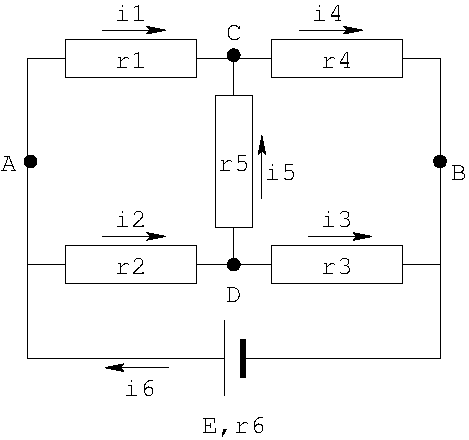
\includegraphics[width=6cm]{wheatstone.pdf}$$
$$
\begin{array}{lcr}
r_1 & = & 10 \Omega \\
r_2 & = & 10 \Omega \\
r_3 & = &  5 \Omega \\
r_4 & = & 20 \Omega \\
r_5 & = & 10 \Omega \\
r_6 & = & 10 \Omega \\
E   & = & 12 V 
\end{array}
\hspace*{5mm}
\left|\begin{array}{l}
i_4 = i_1 + i_5\\
i_6 = i_1 + i_2\\
i_2 = i_3 + i_5\\
10 i_1 = 10 i_2 + 10 i_5\\
10 i_5 = 5 i_3 - 20 i_4\\
12 - 10 i_6 = 10 i_2 + 5 i_3
\end{array}\right.
$$
\end{fig}
}
De nombreux exemples traités dans les enseignements scientifiques
conduisent à la nécessité de résoudre un système de $n$ équations linéaires
à $n$ inconnues, homogènes ou non homogènes, du type $A\cdot x = b$. 
La figure \ref{fig:wheatstone}
propose à titre d'exemple le cas du pont de Wheatstone en électricité.
Les ponts ont été utilisés pour la mesure des résistances, inductances et
capacités jusqu'à ce que les progrès en électronique les rendent obsolètes en
métrologie. Toutefois la structure en pont reste encore utilisée dans de 
nombreux montages (voir par exemple \cite{rousseau07})\label{cite:rousseau}.

La première méthode généralement utilisée pour trouver la solution 
d'un système d'équa\-tions linéaires tel que le système (\ref{eq1}) 
est celle qui consiste à éliminer les inconnues 
($x_i$) en combinant les équations \cite{florent77}\label{cite:florent2}.
Pour illustrer cette méthode, nous commencerons par étudier un exemple
simple pouvant s'effectuer {\em à la main}, 
puis nous passerons au cas général pour
présenter la méthode d'élimination de {\sc Gauss}.

%-------------------------------------------------------------------------
\subsubsection*{Etude d'un cas particulier}
\label{casparticulier}
%-------------------------------------------------------------------------
Considérons le système suivant :
$$\left\{
\begin{array}{rcrcrcr}
 x_0 & + &  x_1 & + &   x_2 & = &  1 \\
2x_0 & + & 4x_1 & + &  8x_2 & = & 10 \\
3x_0 & + & 9x_1 & + & 27x_2 & = & 33
\end{array}
\right.$$

Pour résoudre un tel système, l'idée de base est de triangulariser 
le système de telle manière qu'il soit possible de remonter les
solutions par substitutions successives.

La première étape consiste à éliminer le terme en $x_0$ des 
$2^{\grave eme}$ et $3^{\grave eme}$ équations.
Cherchons tout d'abord à éliminer le terme en $x_0$ de la $2^{\grave eme}$
équation. Pour cela nous multiplions la $1^{\grave ere}$ équation par le 
coefficient de $x_0$ de la $2^{\grave eme}$ équation ($a_{10} = 2$). 
On obtient le nouveau système :
$$\left\{
\begin{array}{rcrcrcr}
2x_0 & + & 2x_1 & + &  2x_2 & = &  2 \\
2x_0 & + & 4x_1 & + &  8x_2 & = & 10 \\
3x_0 & + & 9x_1 & + & 27x_2 & = & 33
\end{array}
\right.$$
On soustrait alors la première équation de la deuxième équation, 
ce qui conduit au système :
$$\left\{
\begin{array}{rcrcrcr}
2x_0 & + & 2x_1 & + &  2x_2 & = &  2 \\
     &   & 2x_1 & + &  6x_2 & = &  8 \\
3x_0 & + & 9x_1 & + & 27x_2 & = & 33
\end{array}
\right.$$
On recommence l'opération pour éliminer le terme en $x_0$ de la $3^{\grave eme}$
équation. Pour cela, on ramène à $1$ le coefficient de $x_0$ dans
la première équation en divisant cette équation par 2 ($a_{00} = 2$),
puis nous multiplions la $1^{\grave ere}$ équation par le 
coefficient de $x_0$ de la $3^{\grave eme}$ équation ($a_{20} = 3$). 
$$\left\{
\begin{array}{rcrcrcr}
3x_0 & + & 3x_1 & + &  3x_2 & = &  3 \\
     &   & 2x_1 & + &  6x_2 & = &  8 \\
3x_0 & + & 9x_1 & + & 27x_2 & = & 33
\end{array}
\right.$$
On soustrait ensuite la $1^{\grave ere}$ équation de la $3^{\grave eme}$ équation :
$$\left\{
\begin{array}{rcrcrcr}
3x_0 & + & 3x_1 & + &  3x_2 & = &  3 \\
     &   & 2x_1 & + &  6x_2 & = &  8 \\
     &   & 6x_1 & + & 24x_2 & = & 30
\end{array}
\right.$$
On obtient un nouveau système linéaire dans lequel seule la première équation contient
un terme en $x_0$.
L'équation utilisée (ici la $1^{\grave ere}$ équation) pour éliminer une inconnue 
dans les équations qui suivent (ici les $2^{\grave eme}$ et $3^{\grave eme}$ équations)
est appelée l'équation-pivot. Dans l'équation-pivot choisie, le coefficient de 
l'inconnue qui est éliminée dans les autres équations est appelé le pivot de
l'équation (ici $a_{00}$).

La deuxième étape consiste à éliminer le terme en $x_1$ de la troisième équation
en utilisant la deuxième équation comme équation-pivot. On ramène à $1$ le coefficient 
de $x_1$ dans la $2^{\grave eme}$ équation en divisant l'équation par 2 ($a_{11} = 2$),
puis on la multiplie par 6 ($a_{21} = 6$) pour que les $2^{\grave eme}$ et 
$3^{\grave eme}$ équations aient le même terme en $x_1$. Tout revient à
multiplier la $2^{\grave eme}$ équation par 3 ($a_{21}/a_{11} = 6/2 = 3$) :
$$\left\{
\begin{array}{rcrcrcr}
3x_0 & + & 3x_1 & + &  3x_2 & = &  3 \\
     &   & 6x_1 & + & 18x_2 & = & 24 \\
     &   & 6x_1 & + & 24x_2 & = & 30
\end{array}
\right.$$
Il reste à soustraire la $2^{\grave eme}$ équation de la $3^{\grave eme}$
pour éliminer le terme en $x_1$ de la $3^{\grave eme}$ équation :
$$\left\{
\begin{array}{rcrcrcr}
3x_0 & + & 3x_1 & + &  3x_2 & = &  3 \\
     &   & 6x_1 & + & 18x_2 & = & 24 \\
     &   &      &   &  6x_2 & = &  6
\end{array}
\right.$$
On obtient ainsi un système triangulaire d'équations linéaires 
dont on peut calculer
directement la valeur de $x_2$ par la $3^{\grave eme}$ équation : $6x_2 =  6 \Rightarrow
x_2 = 1$. On porte cette valeur de $x_2$ dans la deuxième équation, ce qui nous permet de
calculer $x_1$ : $6x_1 + 18\cdot 1 = 24 \Rightarrow x_1 = 1$. En reportant les valeurs de
$x_2$ et $x_1$ dans la première équation, on en déduit la valeur de $x_0$ :
$3x_0 + 3\cdot 1 +  3\cdot 1 =  3 \Rightarrow x_0 = -1$. 
On vérifie simplement que
les valeurs obtenues sont solutions du système initial :
$$\left\{
\begin{array}{rcrcrcr}
 x_0 & + &  x_1 & + &   x_2 & = &  1 \\
2x_0 & + & 4x_1 & + &  8x_2 & = & 10 \\
3x_0 & + & 9x_1 & + & 27x_2 & = & 33
\end{array}
\right.
\hspace*{2cm}
\left(
\begin{array}{rrr}
1 & 1 &  1 \\
2 & 4 &  8 \\
3 & 9 & 27 
\end{array}
\right)
\cdot
\left(
\begin{array}{r}
-1 \\ 1 \\ 1
\end{array}
\right)
=
\left(
\begin{array}{r}
1 \\ 10 \\ 33
\end{array}
\right)$$

%-------------------------------------------------------------------------
\subsubsection*{Etude du cas général}
\label{casgeneral}
%-------------------------------------------------------------------------
De manière générale, la méthode précédente consiste à réduire le système de $n$ 
équations à $n$ inconnues à un système triangulaire équivalent qui peut 
être ensuite résolu facilement par substitutions. En quelque sorte le système 
(\ref{eq1}) doit être transformé en un système équivalent du type :
\begin{equation}\label{eq2}
\left\{
\begin{array}{rcrcrcrcr@{\ =\ }r}
a_{00}x_0 &+& a_{01}x_1       &+& a_{02}x_2       &+& \cdots &+& a_{0(n-1)}x_{(n-1)}       & b_0\\
          & & a^{(1)}_{11}x_1 &+& a^{(1)}_{12}x_2 &+& \cdots &+& a^{(1)}_{1(n-1)}x_{(n-1)} & b^{(1)}_1\\
          & &                 &+& a^{(2)}_{22}x_2 &+& \cdots &+& a^{(2)}_{2(n-1)}x_{(n-1)} & b^{(2)}_2\\
          & &                 & &                 & & \cdots &+& \cdots           & \cdots\\
          & &                 & &                 & &        & & a^{(n-2)}_{(n-1)(n-1)}x_{(n-1)}   & b^{(n-2)}_{(n-1)}
\end{array}
\right.
\end{equation}
où l'indice supérieur désigne le nombre d'étapes à la suite desquelles est obtenu le 
coefficient considéré.

L'équation de rang 0 du système (\ref{eq1}) est d'abord divisée par le coefficient 
$a_{00}$ de $x_0$ (supposé non nul). On obtient :
\begin{equation}\label{eq3}
x_0 + \frac{a_{01}}{a_{00}}x_1 + \frac{a_{02}}{a_{00}}x_2 + \cdots + \frac{a_{0(n-1)}}{a_{00}}x_{(n-1)} = \frac{b_0}{a_{00}}
\end{equation}
Cette équation (\ref{eq3}) est alors multiplié par $a_{10}$, coefficient de $x_0$ dans 
la deuxième équation du système (\ref{eq1}). Le résultat est ensuite soustrait de la 
deuxième équation du système (\ref{eq1}), ce qui élimine $x_0$ dans la deuxième équation.
D'une manière générale on multiplie la relation (\ref{eq3}) par $a_{i0}$, coefficient
de $x_0$ dans l'équation de rang $i$ du système (\ref{eq1}) et on retranche le résultat
obtenu de cette même $i^{\grave eme}$ équation. A la fin $x_0$ est éliminé de toutes les équations, excepté de la première, et on obtient le système ainsi transformé :
\begin{equation}\label{eq4}
\left\{
\begin{array}{rcrcrcrcr@{\ =\ }r}
a_{00}x_0 &+& a_{01}x_1       &+& a_{02}x_2       &+& \cdots &+& a_{0(n-1)}x_{(n-1)}       & b_0\\
          & & a^{(1)}_{11}x_1 &+& a^{(1)}_{12}x_2 &+& \cdots &+& a^{(1)}_{1(n-1)}x_{(n-1)} & b^{(1)}_1\\
          & & a^{(1)}_{21}x_1 &+& a^{(1)}_{22}x_2 &+& \cdots &+& a^{(1)}_{2(n-1)}x_{(n-1)} & b^{(1)}_2\\
          & & a^{(1)}_{31}x_1 &+& a^{(1)}_{32}x_2 &+& \cdots &+& a^{(1)}_{3(n-1)}x_{(n-1)} & b^{(1)}_3\\
          & & \cdots          &+& \cdots          &+& \cdots &+& \cdots                    & \cdots\\
          & & a^{(1)}_{(n-1)1}x_1 &+& a^{(1)}_{(n-1)2}x_2 &+& \cdots &+& a^{(1)}_{(n-1)(n-1)}x_{(n-1)}   & b^{(1)}_{(n-1)}
\end{array}
\right.
\end{equation}
L'équation de rang 1 dans le nouveau système (\ref{eq4}) devient alors l'équation-pivot
et $a^{(1)}_{11}$ le pivot de l'équation. De la même façon on élimine $x_1$ des
équations du rang $2$ au rang $n-1$ dans le système (\ref{eq4}), et on obtient :
\begin{equation}\label{eq5}
\left\{
\begin{array}{rcrcrcrcr@{\ =\ }r}
a_{00}x_0 &+& a_{01}x_1       &+& a_{02}x_2       &+& \cdots &+& a_{0(n-1)}x_{(n-1)}       & b_0\\
          & & a^{(1)}_{11}x_1 &+& a^{(1)}_{12}x_2 &+& \cdots &+& a^{(1)}_{1(n-1)}x_{(n-1)} & b^{(1)}_1\\
          & &                 & & a^{(2)}_{22}x_2 &+& \cdots &+& a^{(2)}_{2(n-1)}x_{(n-1)} & b^{(2)}_2\\
          & &                 & & a^{(2)}_{32}x_2 &+& \cdots &+& a^{(2)}_{3(n-1)}x_{(n-1)} & b^{(2)}_3\\
          & &                 & & \cdots          &+& \cdots &+& \cdots                    & \cdots\\
          & &                 & & a^{(2)}_{(n-1)2}x_2 &+& \cdots &+& a^{(2)}_{(n-1)(n-1)}x_{(n-1)}   & b^{(2)}_{(n-1)}
\end{array}
\right.
\end{equation}
L'équation de rang 2 dans le nouveau système (\ref{eq5}) fait office à son tour d'équation
pivot, et ainsi de suite jusqu'à obtenir le système triangulaire (\ref{eq2}).
Une fois obtenu ce système triangulaire, on calcule directement
la valeur de $x_{(n-1)}$ par la dernière relation du système triangulaire. 
En portant cette valeur dans la relation précédente, on calculera
$x_{(n-2)}$, et ainsi de suite en remontant le système triangulaire (\ref{eq2}).
A chaque étape $k$, on a donc les relations suivantes :
\begin{enumerate}
\item {Triangularisation}
	$$\left\{
	\begin{array}{lcl}
	a_{ij}^{(k)} & = & \displaystyle a_{ij}^{(k-1)} - \frac{a_{ip}^{(k-1)}}{a_{pp}^{(k-1)}}\cdot
	a_{pj}^{(k-1)} \\[5mm]
	b_i^{(k)}    & = & \displaystyle b_i^{(k-1)} - \frac{a_{ip}^{(k-1)}}{a_{pp}^{(k-1)}}\cdot
	b_p^{(k-1)}
	\end{array}
	\right.\mbox{\footnotesize\ avec\ }
	\left\{
	\begin{array}{l}
	k\ :\ \mbox{\footnotesize étape}\\
	p\ : \ \mbox{\footnotesize rang du pivot}\\[5mm]
	p < i \leq (n-1) \\[2mm]
	p \leq j \leq (n-1)
	\end{array}
	\right.$$
\item {Remontée par substitutions} 
	$$\left\{
	\begin{array}{lcl}
	x_{(n-1)} & = & \displaystyle\frac{b_{(n-1)}}{a_{(n-1)(n-1)}}\\[5mm]
	x_i       & = & \displaystyle\frac{\displaystyle b_{i} - 
	\sum_{j=i+1}^{n-1} a_{ij}x_j}{a_{ii}} 
	\end{array}
	\right.
	\mbox{\ avec\ } 0 \leq i < (n-1)$$
\end{enumerate}

\marginpar{\footnotesize\em
\begin{rem}
Cette méthode est connue sous le nom de méthode d'élimination 
de {\sc Gauss} (également connue sous
le nom de méthode de triangularisation de {\sc Gauss} ou méthode du pivot 
de {\sc Gauss}). Elle fut nommée ainsi en l'honneur du mathématicien allemand 
{\sc Johann Carl Friedrich Gauss} (1777--1855), mais elle est connue des Chinois 
depuis au moins le $1^{er}$ siècle de notre ère. Elle est référencée dans le livre 
chinois « Jiuzhang suanshu~» où elle est attribuée à {\sc Chang Ts'ang} chancelier de 
l'empereur de Chine au $2^{\grave eme}$ siècle avant notre ère \cite{chemla04}\label{cite:chemla}.
\end{rem}
}
Jusqu'à présent, on a admis que le pivot au cours du processus de triangularisation 
était non nul ($a_{pp} \neq 0$). Si ce n'est pas le cas, on doit permuter 
l'équation-pivot avec une autre ligne dans laquelle le pivot est différent de 0.
Il se peut également que le pivot, sans être nul, soit très petit et l'on a 
intérêt là-aussi à interchanger les lignes comme pour le cas d'un pivot nul.
En fait, pour augmenter la précision de la solution obtenue, on a toujours 
intérêt à utiliser la ligne qui a le plus grand pivot.

%-------------------------------------------------------------------------
\subsubsection*{Jeu de tests}
\label{casgeneral}
%-------------------------------------------------------------------------
L'algorithme de résolution de tels systèmes linéaires pourra être testé
à l'aide des systèmes suivants :
$$\begin{array}{|l|c|c|c|}
\hline
\mbox{\bf Test} & \multicolumn{2}{|c|}{\mbox{{\bf Système} $A\cdot x = b$}} & \bf Solution\\
\cline{2-3}
                & A & b & \bf exacte \\
\hline
\hline
1 
& 
\left(\begin{array}{r}
4
\end{array}\right) 
&
\left(\begin{array}{r}
1
\end{array}\right) 
&
\displaystyle
\left(\begin{array}{r}
1/4
\end{array}\right)\\
\hline
2 
& 
\left(\begin{array}{rr}
1 & 1 \\
1 & -1
\end{array}\right) 
&
\left(\begin{array}{r}
1 \\ 0
\end{array}\right)
&
\displaystyle
\left(\begin{array}{r}
1/2 \\ 1/2
\end{array}\right)
\\
\hline
3 
& 
\left(\begin{array}{rrr}
2 & -1 & 2 \\
1 & 10 & -3 \\
-1 & 2 & 1
\end{array}\right) 
&
\left(\begin{array}{r}
2 \\ 5 \\ -3
\end{array}\right)
&
\left(\begin{array}{r}
2 \\ 0 \\ -1
\end{array}\right)
\\
\hline
\end{array}$$


$$\begin{array}{|l|c|c|c|}
\hline
\mbox{\bf Test} & \multicolumn{2}{|c|}{\mbox{{\bf Système} $A\cdot x = b$}} & \bf Solution\\
\cline{2-3}
                & A & b & \bf exacte \\
\hline
4 &
\left(\begin{array}{rrrr}
10 & 7 & 8 & 7 \\
7 & 5 & 6 & 5 \\
8 & 6 & 10 & 9 \\
7 & 5 & 9 & 10
\end{array}\right) 
&
\left(\begin{array}{r}
32 \\ 23 \\ 33 \\ 31
\end{array}\right) 
&
\left(\begin{array}{r}
1 \\ 1 \\ 1 \\ 1
\end{array}\right) 
\\
\hline
5 & 
\left(\begin{array}{rrrr}
10 & 7 & 8.1 & 7.2 \\
7.08 & 5.04 & 6 & 5 \\
8 & 5.98 & 9.89 & 9 \\
6.99 & 4.99 & 9 & 9.98
\end{array}\right) 
&
\left(\begin{array}{r}
32 \\ 23 \\ 33 \\ 31
\end{array}\right) 
&
\mbox{---} \\
\hline
6 &
\left(\begin{array}{rrrr}
10 & 7 & 8 & 7 \\
7 & 5 & 6 & 5 \\
8 & 6 & 10 & 9 \\
7 & 5 & 9 & 10
\end{array}\right) 
&
\left(\begin{array}{r}
32.01 \\ 22.99 \\ 33.01 \\ 30.99
\end{array}\right) 
&
\mbox{---} \\
\hline
\end{array}$$
\marginpar{\footnotesize\em
\begin{rem}
Les tests 5 et 6 sont des variations du test 4 : $A_5 = A_4 + \Delta A$
et $b_6 = b_4 + \Delta b$. Ces 2 tests sont effectués pour évaluer 
les conséquences sur la solution $x$ d'une perturbation $\Delta A$ de $A_4$
et d'une perturbation $\Delta b$ de $b_4$.
$$\Delta A = \left(\begin{array}{rrrr}
0 & 0 & 0.1 & 0.2\\
0.08 & 0.04 & 0 & 0\\
0 & -0.02 & -0.11 & 0\\
-0.01 & -0.01 & 0 & -0.02
\end{array}
\right)$$
$$\Delta b = \left(\begin{array}{r}
0.01 \\ - 0.01 \\ 0.01 \\ -0.01
\end{array}\right)$$
Le test 7 correspond à l'exemple du pont de Wheatstone 
(figure \ref{fig:wheatstone}). Le test 8 correspond
à la détermination de la forme d'une came rotative qui doit
mettre en mouvement un axe suivant une loi horaire donnée
(exemple tiré de \cite{florent77}).
\end{rem}
}

$$\begin{array}{|l|c|c|}
\hline
\mbox{\bf Test} & \multicolumn{2}{|c|}{\mbox{{\bf Système} $A\cdot x = b$}}\\
\cline{2-3}
                & A & b  \\
\hline
\hline
7 &
\left(\begin{array}{rrrrrr}
1 & 0 & 0 & - & 1 & 0\\
1 & 1 & 0 & 0 & 0 & -1\\
0 & 1 & -1 & 0 & -1 & 0\\
10 & -10 & 0 & 0 & -10 & 0\\
0 & 0 & 5 & -20 & -10 & 0\\
0 & 10 & 5 & 0 & 0 & 10
\end{array}\right) 
&
\left(\begin{array}{r}
0 \\ 0 \\ 0 \\ 0 \\ 0 \\ 12
\end{array}\right)\\
\hline
8 &
\left(\begin{array}{rrrrrrrr}
1 & 0 & 0 & 0 & 0 & 0 & 0 & 0\\
1 & 2\pi & 4\pi^2 & 8\pi^3 & 16\pi^4 & 32\pi^5 & 64\pi^6 & 128\pi^7\\
0 & 1 & 0 & 0 & 0 & 0 & 0 & 0\\
0 & 1 & 4\pi & 12\pi^2 & 32\pi^3 & 80\pi^4 & 192\pi^5 & 448\pi^6\\
1 & \pi/2 & \pi^2/4 & \pi^3/8 & \pi^4/16 & \pi^5/32 & \pi^6/64 & \pi^7/128\\
0 & \pi/2 & \pi & 3\pi^2/4 & \pi^3/2 & 5\pi^4/16 & 3\pi^5/16 & 7\pi^6/64\\
1 & \pi & \pi^2 & \pi^3 & \pi^4 & \pi^5 & \pi^6 & \pi^7\\
0 & \pi & 2\pi & 3\pi^2 & 4\pi^3 & 5\pi^4 & 6\pi^5 & 7\pi^6
\end{array}\right) 
&
\left(\begin{array}{r}
4 \\ 4 \\ 0 \\ 0 \\ 2 \\ -2 \\ 1 \\ 0
\end{array}\right)\\
\hline
\end{array}$$

